\documentclass[a4paper, man, natbib, floatsintext]{apa6} %jou, man, report, doc

\usepackage{standalone}
\usepackage[english]{babel}
\usepackage[utf8x]{inputenc}
\usepackage{amsmath,amssymb}
\usepackage{graphicx}
\usepackage[colorinlistoftodos]{todonotes}

\usepackage{multicol}
\usepackage{multirow}
\usepackage{booktabs} %booktabs package makes nice tables!
\usepackage{url}
\usepackage{rotating}
\usepackage[toc,page]{appendix}
\usepackage{color}
\usepackage{subscript}
\usepackage{threeparttable}
\usepackage{threeparttablex}
\usepackage{longtable}
\usepackage{times}
\usepackage{upgreek}
\AtBeginEnvironment{tabular}{\onehalfspacing}

%% For the revision
\usepackage{changes}
\definechangesauthor[name={JJ}, color=orange]{jj}
%% Use "final" option to remove all tracking markups
% \usepackage[final]{changes}

%\usepackage[style=apa,sortcites=true,sorting=nyt,backend=biber]{biblatex}
%\addbibresource{/Users/jhoffart/Documents/Dropbox/Basel/References/refJanine.bib}
%\addbibresource{refJanine.bib}


\title{The influence of sample size on preferences from experience}
\shorttitle{sample size and preference}

\author{Janine Christin Hoffart\\J\"org Rieskamp\\Gilles Dutilh}
\affiliation{University of Basel, Department of Psychology, Center for Economic Psychology}

\leftheader{Hoffart, Rieskamp, Dutilh}

\abstract{\textcolor{blue}{People often evaluate risky options in situations in which they need to learn from experience how likely the options' outcomes are. When people can actively sample information about outcomes and outcome probabilities to make decisions, they typically draw small samples. To understand why people rely on small samples, we studied how the amount of information influences preferences for gambles. In two studies, people drew samples of different sizes from risky gambles and then indicated their selling prices for these gambles and their confidence in their judgments. Remarkably, the results show that averaged across people, neither valuations nor confidence in the valuations changed substantially with sample size. However, on an individual level approximately half of the participants could be classified as Bayesian learners and the other half as frequentist learners. Valuations of Bayesian learners changed with sample size as predicted by Bayesian principles. In contrast, sample size did not influence valuations of frequentist learners. These results illustrate the variability in how people learn from sampled information and provide an explanation for why sample size often does not affect judgments. 
}} 


\keywords{D--E gap, valuations from experience}
\authornote{This research is supported by a grant (SNF \# 143854) from the Swiss National Science Foundation to the second and third author. We thank Anita Todd for editing the manuscript. 

Correspondence concerning this article should be addressed to Janine Christin Hoffart, University of Basel, Department of Psychology, Missionsstrasse 62a, 4055 Basel, Switzerland.  E-mail: janine.hoffart@unibas.ch}

\begin{document}
\maketitle

In everyday life, people often form preferences on the basis of past experiences. How strong these preferences are arguably depends on the amount of previous experience. Someone who has visited a restaurant for many years and has always had positive experiences likely has a stronger positive preference for this restaurant than someone who visited the restaurant only once and had a positive experience. Thus, even if the relative frequency of positive experiences is similar, the strength of preferences can differ. We examined how people's preferences in an experience-based judgment situation evolve as a function of growing experience. 

%In everyday life people often base their preferences on past experiences. How much experience people have made with an option arguably influences how strong people's opinion about this option is. Someone who had made 50 out of 50 good experiences with a restaurant probably has a stronger preference for this restaurant than someone who had made 1 out of 1 good experience with this restaurant although the relative frequency of good experiences is the same in both situations. Here, we study, how people's preferences (i.e. valuations) in an experience-based task evolve as a function of growing experience. 

\section{The D--E Gap and Search Effort in Experience-Based Tasks}
How people develop preferences on the basis of information that they accumulate over time has been studied with experience-based judgment and decision-making tasks \citep[e.g.,][]{Hertwig2004, Hau2008}. %Recently, there has been developing growing interest in studying experience based tasks \citep[e.g.][]{Hertwig2004, Hau2008}. 
Experience-based tasks differ from descriptive tasks in the way information is presented. In descriptive tasks, people make judgments about gambles according to numerical, graphical, or text-based summaries of the gambles' outcome distributions. In experience-based tasks, on the other hand, people learn about the outcome distributions by repeatedly drawing samples from them until they feel confident to make a judgment or decision. Interestingly, past research suggests that people's decisions systematically differ between description- and experience-based tasks (the so-called D--E gap): When people make decisions from description, they choose as if they overweight rare events \citep{Kahneman1979}. At the same time, when they make similar decisions on the basis of experience, they choose as if they underweight rare events \citep{Hertwig2004}. 

%\subsection{Sample size in experience--based tasks}
The D--E gap has often been attributed to limited search effort in experience-based tasks and resulting \textit{sampling error}. Such sampling error occurs when the observed outcome sequence deviates from the objective outcome probabilities \citep{Hadar2009}. For instance, \cite{Hertwig2004} reported that participants drew a median of only 15 observations per decision. With such a low number, the skew of a gamble's binomial sampling distribution implies that more people undersample than oversample a rare event. Indeed, averaged across trials, in Hertwig et al.'s study, the rare event was undersampled by $78\%$ of the participants. Other studies have reported similar sampling errors \citep[e.g.,][]{Hau2008,Rakow2008}. \textcolor{blue}{Explanations for why people often search insufficiently are manifold. Limited memory capacity may impede excessive information search, and extensive search may not be justified when opportunity costs are high \citep{Hau2008}. A slightly different explanation suggests that by relying on small sample sizes, people simplify their choices \citep{Hertwig2010}: Simulation studies have shown that when people compare two outcome distributions on the basis of sampling from them, small sample sizes amplify the differences between the observed means.}

Since the initial finding that people often sample insufficiently, researchers have tried to reduce or eliminate sampling error. Attempts have involved encouraging participants to draw larger samples by increasing the incentives \citep{Hau2008}; showing fixed samples that represent the gambles' objective probability distributions \citep{Ungemach2009}; showing fixed---relatively large---numbers of random samples, as larger total samples naturally reduce sampling error \citep{Hau2008,Hau2010}; presenting gamble descriptions that match the outcome distribution that a ``partner'' participant had sampled \citep{Rakow2008}; and constraining statistical analysis to trials in which the total sample closely represents the gambles' underlying outcome distributions \citep[e.g.,][]{Camilleri2009, Camilleri2011a}. Typically, the goal of the attempt to eliminate sampling error was to allow for an unbiased comparison between decisions from description and decisions from experience. The results are mixed: In some studies, the authors found a diminished D--E gap \citep{Hau2008,Hau2010, Ungemach2009} or failed to find a D--E gap \citep{Gloeckner2012, Camilleri2009,Camilleri2011a,Rakow2008}. \textcolor{blue}{Yet, despite these mixed findings, the robustness of the gap was confirmed in a recent meta-analysis \citep{Wulff2017}.}

While the question of whether people process information from description differently from information from experience is of great importance, in the present work, we approached it only marginally. Instead, we examined how valuations of risky prospects from experience are influenced by different sample sizes. To do so, we manipulated how many samples people could draw from the prospects' outcome distributions and measured people's preferences (i.e., selling prices).


%While the question whether people process information from description differently than information from experience is definitely interesting, here . Instead we will focus on how sample size influences how risky prospects are evaluated. To do so, we manipulate how many samples people can draw from the prospects' outcome distributions and study whether sample size influences preferences.

\section{How Does Sample Size Influence Preferences?}
The question of how sample size influences judgments has interested psychologists for decades \citep[e.g.,][]{Tversky1971, Griffin1992}. We investigated how sample size influences preferences from experience, by contrasting two existing theories: \textit{the belief in the law of small numbers} \citep{Tversky1971} and \textit{Bayesian updating}. 

\subsection{Belief in the Law of Small Numbers}
\cite{Tversky1971} formulated the belief in the law of small numbers: an exaggerated belief about the likelihood of small sequences of random draws representing outcome distributions. % Evidence for this belief has 
For instance, when people were asked to mentally produce a short sequence of random coin tosses, the produced sequences resembled a relative frequency of $.5$ more often than expected by chance \citep{Tversky1971}. \cite{Griffin1992} showed that people tend to neglect the role of sample size in their judgments. \textcolor{blue}{Participants in an experiment saw sequences of coin tosses and then estimated the probability that a coin was biased and expressed their confidence in their estimate. The researchers varied the total number of coin tosses (i.e., sample size) and---unbeknownst to the participants---used coins with different biases.} \cite{Griffin1992} found that participants neglected sample size and based their estimates mostly on the observed relative frequency of head and tail outcomes. Surprisingly, participants expressed more confidence in their judgments when the number of coin tosses was small. Since these initial findings, several studies have confirmed that people are often less sensitive to sample size than normative models suggest \textcolor{blue}{in inferential judgment tasks \citep[e.g.,][]{Kutzner2016}, perceptual judgment tasks \citep[e.g.,][]{Kvam2016}, and also preferential tasks \citep[e.g.,][]{Powell2017}.}  

\subsection{Bayesian Updating}

In contrast to the psychological principle of the belief in the law of small numbers, Bayesian principles suggest that sample size influences judgments. 
The Bayesian view offers a normative solution to how people deal with sample sizes. People can treat sample size as a measure of uncertainty, knowing that small samples can lead to a biased representation of the true outcome distribution and larger samples to a more veridical description of the true outcome distribution. Recent research has provided evidence that people indeed treat sample size as a measure of uncertainty, for instance, when they report preferences for consumer goods \citep{DeMartino2017} or make judgments about group differences \citep{Obrecht2010} or the performance of students \citep{Fiedler2002}.

\subsection{Cognitive Models and Hypothesis}
To investigate how people deal with accumulating evidence, we tested whether they integrate samples by following Bayesian principles or by following the belief in the law of small numbers. For this purpose, we formalized two models that mathematically implement the two theories described above. 


To understand the models, it is crucial to recognize the following facts about our experimental methods. In our experiments, we asked participants to indicate their valuations (i.e., selling prices) of two-outcome gambles where one of the outcomes was always 0. People were able to sample a \textit{predefined} number of outcomes from the gamble's outcome distribution and then indicated their selling price for this gamble. Because there were only two outcomes, of which one was always 0, the following models were defined by estimating the probability of the nonzero gain outcome. Note that extensions of the models for more general cases with several outcomes are possible. Importantly, the sample sequences that people saw were always representative of the gamble's outcome distribution. Individual gambles were presented with different sample sizes. 

Both models that we propose are expected utility models. According to expected utility theory, people's preferences about risky options can be represented by subjective utility functions. The subjective value of a risky option is defined as the sum of \textcolor{blue}{the subjective utilities of the outcomes weighted by the outcome probabilities. To allow for monetary evaluations of an option the expected utility is then converted back to the monetary scale}. If outcome probabilities are not provided, as in experience-based tasks, they can be replaced by the decision makers' beliefs. Crucially, the two models that we propose differ with regard to how people develop beliefs about the outcome probabilities.

\subsubsection{Relative frequency model}

\added[id=jj]{The \textit{relative frequency model (RF)} estimates probabilities from relative frequencies. It formalizes how people who trust in the law of small numbers---that frequencies in small samples represent population probabilities---estimate probabilities given different sample sizes.} It suggests that the probabilities of gains is estimated from the relative frequency of observed gains. The relative frequency model predicts that the belief about the gain probability after sampling $t$ times is
$${B}_{\mathrm{RF}, t}  =  \frac{1}{t} \times n_t,$$
\added{where $n_t$ represents the number of gains observed until $t$.}

\added{Critically, the relative frequency model predicts that changes in sample size do not influence valuations. It also predicts that only the sampled outcome frequency influences the estimated probabilities.}

\subsubsection{Bayesian value updating model}
The \emph{Bayesian value updating (BVU)} model  implements a Bayesian perspective on probability estimation and how people deal with uncertainty from sampling. Accordingly, peoples' beliefs about the gain probabilities follow Bayesian principles. \added[id=jj]{Unlike the relative frequency model, the Bayesian model highlights the role of prior beliefs about outcome probabilities before sampling. The beliefs about gain probabilities follow a beta distribution ${B}_{\mathrm{BVU}} \sim Beta(a,b)$. Before sampling, at $t = 0$, the beliefs are represented by a prior belief distribution $B_{\mathrm{BVU},0} \sim Beta(\theta_G$, $\theta_0)$, which is person-specific. The prior belief is updated from the sampled number of gains and zero-outcomes. The updated beliefs after sampling $t$ times follow the distribution}

$$B_{\mathrm{BVU},t} \sim Beta(\theta_G + \delta a_t, \theta_0 + \delta b_t)$$,

where  $\delta$ is a learning rate to account for individual differences in conservatism \citep{Edwards}, $a_t, b_t$ are the counts of gains and zero-outcomes (respectively) after sample $t$, and $\theta_G$, $\theta_0$ are the gain and zero-outcome priors, respectively. The point estimate for the gain probability is the posterior mean of this distribution, ${B}_\mathrm{BVU, t} = \frac{A}{A + B}$, with $A$ being a short-hand for $\theta_G + \delta a_t$ (and respectively for B). \textcolor{blue}{The updating process is illustrated in Figure \ref{fig:sensi} (see also below).}

\subsubsection{Utility Function}
\added[id=jj]{Both, the relative frequency model and Bayesian value updating model, capture individual differences in utility of monetary gamble outcomes by a one-parameter power utility function, $u(g) = g^{\mathrm{\alpha}}$, where $g$ is the gain outcome. Thus, the predicted evaluation by the relative frequency (RF) and Bayesian updating (BVU) model after sample $t$ is given by }

$$V_{\mathrm{RF}, t} = \sqrt[\mathrm{\alpha}]{{B}_{\mathrm{RF}, t} \times u({g})}$$

$$V_{\mathrm{BVU}, t} = \sqrt[\mathrm{\alpha}]{{B}_{\mathrm{BVU}, t} \times u({g})}$$


Following \cite{Griffin1992}, we also asked participants for their confidence in their valuations. We tested whether people would be more confident about their responses when the sample size was small, as found by \cite{Griffin1992}. 

\textcolor{blue}{Figures \ref{fig:sensi}b  and c illustrate how prior beliefs change as people observe new samples. The black curves illustrate how the beliefs change after observing few outcomes (5) with a reward frequencies of 1/5 (20\%, Figure \ref{fig:sensi}b)  and 4/5 (80\%, Figure \ref{fig:sensi}c). The gray curves illustrate how the beliefs change after observing many outcomes (30) with similar reward frequencies.}


Figure \ref{fig:sensi}a illustrates these prior beliefs.
\begin{figure}[htbp] 
  \centering
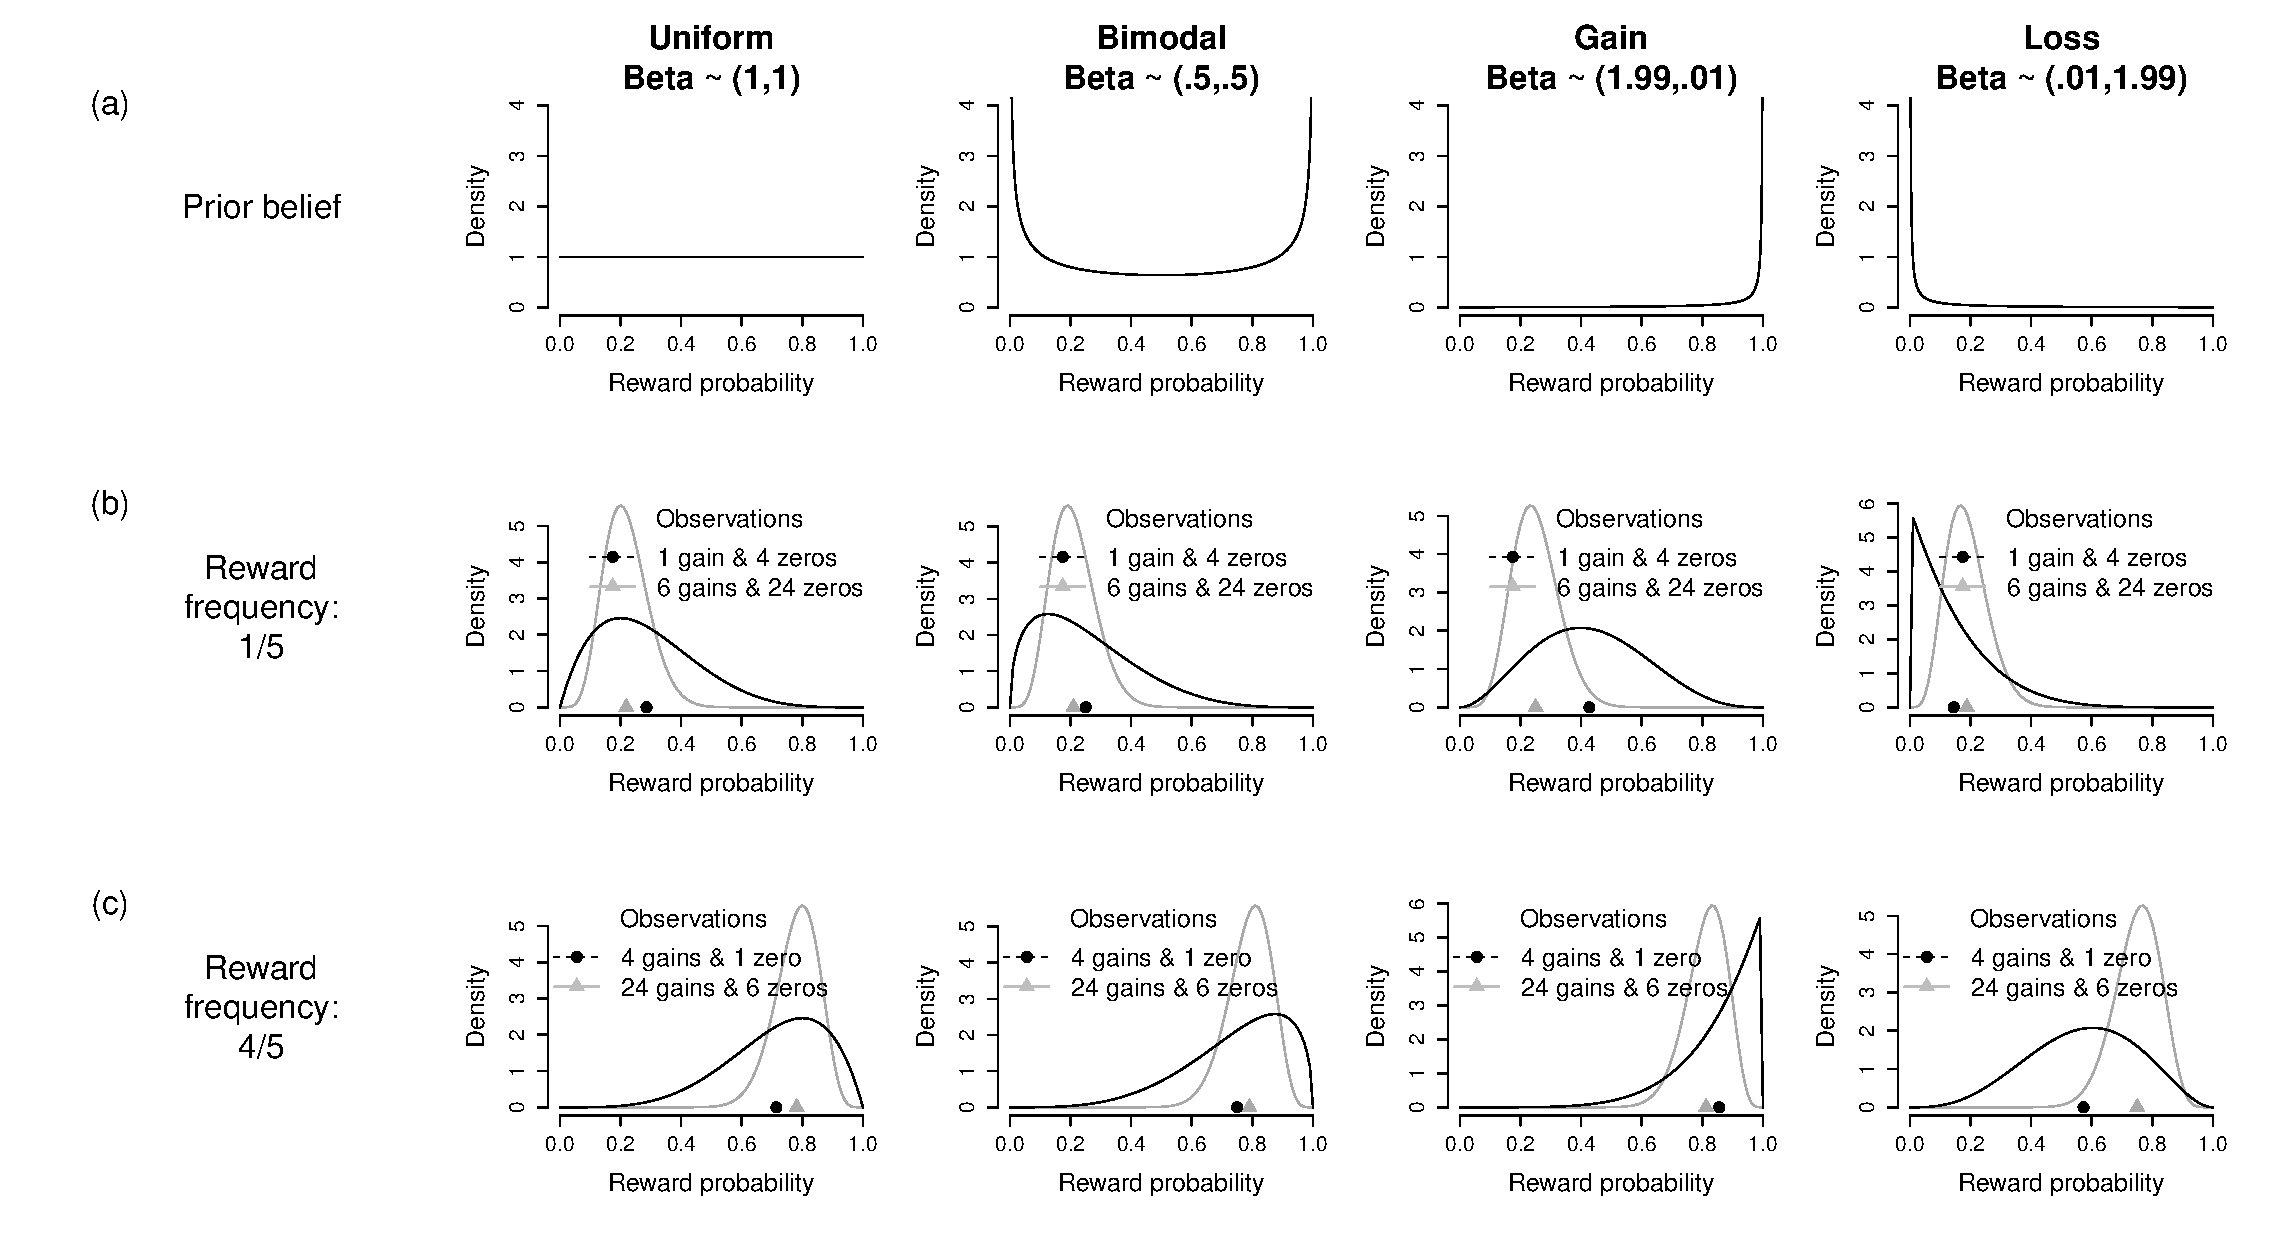
\includegraphics[width=1\linewidth, keepaspectratio]{sensi1.eps}
  \caption{\textcolor{blue}{Every column describes how a specific prior belief (a) gets updated to a posterior belief (b and c). (a) Four different prior beliefs. The titles display the parameters of the beta distributions that created these prior beliefs. (b) Posterior beliefs after observing 5 (black) and 30 (gray) outcomes with a relative reward frequency of one reward per five outcomes (20\%). (c) Posterior beliefs after observing 5 (black) and 30 (gray) outcomes with a relative reward frequency of four rewards per five outcomes (80\%).}}
  \label{fig:sensi}
\end{figure}




The BVU model predicts that sample size influences valuations. This is because as sample size increases, the beta-distributed belief shifts from the \textcolor{blue}{mean of the prior belief (see Figure \ref{fig:sensi}a) in the direction of the true underlying probability of the gain. Whether the model predicts a decrease or an increase in valuations as a function of sample size depends on the shape of the prior belief and the true gain probability. If the gain probability is lower than 50\% and the prior belief is uniform, bimodal, or peaked over gains, the model predicts that valuations decrease as a function of sample size. However, if the prior belief is more peaked over losses, the model predicts that valuations increase as a function of sample size. If the gain probability is larger than 50\% and the prior belief is uniform, bimodal, or peaked over losses, the model predicts that valuations increase as a function of sample size. However, if the prior belief is more peaked over gains, the model predicts that valuations decrease as a function of sample size. In all cases}, the probability belief gets increasingly peaked around the true probability of the gain as sample size grows. Therefore, the model also predicts that confidence in valuations increases with increasing sample size. %We also test this prediction by assessing confidence ratings.

\section{Study 1}
We defined two main goals and one subordinate goal for the experimental method of Studies 1 and 2. First, we aimed to measure people's strength of preference. Therefore, we prompted participants to value single gambles. This approach is in line with recent studies \citep[e.g.,][]{Ashby2014, Golan2014, Pachur2012} and offers the advantage of measuring preference more precisely than with choices. This is important, as detecting subtle differences in strength of preference requires fine-grained measurement scales. Second, we aimed to lay bare the precise effects of sample size. Therefore, we presented each gamble with various sample sizes. To allow for an unbiased comparison of different sample sizes, we eliminated sampling error by presenting representative samples. However, the order of individual samples within a sequence was random.

As as third, subordinate goal we sought to clearly compare valuations from experience with valuations from description. Therefore, we added a block where people made valuations from description. However, as our main goals involved studying how preferences change as a function of sample size, we refrained from manipulating the order of the experience and description blocks. Instead, all people made valuations first from experience and afterward in a separate block from description. 

In Study 1, we examined how people form valuations from experience when they know the possible outcomes before they start sampling. In a situation where the outcomes are known, learning is simplified because participants only need to learn the outcome probabilities from experience. 

\subsection{Method}
\subsubsection{Participants}
Forty people (31 women, 9 men) from the participant pool of the University of Basel between 18 and 40 years old ($M = 23.41$ years, $SD = 4.86$) participated in the study. Participants could choose between a show-up fee of 10 CHF (approximately \$11.10 at the time of the experiment) or course credit. Additionally, each participant received a bonus payment that depended on the outcome of a randomly selected trial ($M = \$6.38$, $SD = \$7.62$).
\subsubsection{Stimuli and Design}
\textcolor{blue}{The design was a within-subject design, participants evaluated two-outcome gambles from experience and then from description. Six gambles were created by crossing two gamble types (\textit{\$-bet}, \textit{p-bet}, see below) with three expected values (2.00, 3.20, 4.00), see Table \ref{table:Lotteries}. Gambles offered a gain or zero, three gambles were \$-bet gambles offering a high gain with low probability, the other three were p-bet gambles offering a small gain with high probability (notation following \citealp{Lichtenstein1971}). In the experience-based evaluation each gamble was crossed with four sample sizes (xs, s, m, l). }

\textcolor{blue}{In the experience condition, we manipulated the sample sizes with which the gambles were presented within-subject, see Table \ref{table:Lotteries}. Four sample size categories were used: extra small (xs = 5, 6, or 7), small (s = xs $\times$ 2), medium (m = xs $\times$ 3), and large (l = xs $\times$ 6). These sample sizes allowed us to represent rare events of 20\% (1/5), roughly 17\% (1/6), and roughly 14\% (1/7). Participants saw each gamble three times with each sample-size, 12 times in total, in fully randomized order.} %For illustration of the different sample sizes, consider Gamble 1 in Table~\ref{table:Lotteries}. It is a \$-bet that offers a gain of 16 with a probability of 1/5 (20\%). The different sample-size categories for this gamble are xs (five observations, one gain), s (ten observations, two gains), m (15 observations, three gains), and l (30 observations, six gains).}

\textcolor{blue}{To avoid memory effects between trials, 18 filler trials were shown, that involved six gambles with outcomes identical to Table~\ref{table:Lotteries}, but probabilities changed to 75\% (\$-bets) and 25\% (p-bets). The filler gambles' sample sizes were 4, 8, and 16. Filler trials were excluded from analyses, because they only aimed at minimizing memory-effects.}

\begin{table}[bth]
\begin{center}
\begin{threeparttable}
\caption{Gambles and Sample Sizes Used in Studies 1 and 2\label{table:Lotteries}}
\begin{tabular}{llccccccc}
\toprule
 &  &  &  &  & \multicolumn{4}{c}{Sample Size} \\
\cmidrule(r){6-9}
Gamble ID & Type & X & Pr & EV & xs & s & m & l\\
\midrule
1 & \$-bet & 16.00 & 0.20 & 3.20 & 5 & 10 & 15 & 30\\
2 & \$-bet & 12.00 & 0.17 & 2.00 & 6 & 12 & 18 & 36\\
3 & \$-bet & 28.00 & 0.14 & 4.00 & 7 & 14 & 21 & 42\\
4 & p-bet & 4.00 & 0.80 & 3.20 & 5 & 10 & 15 & 30\\
5 & p-bet & 2.40 & 0.83 & 2.00 & 6 & 12 & 18 & 36\\
6 & p-bet & 4.70 & 0.86 & 4.03 & 7 & 14 & 21 & 42\\
\bottomrule
\addlinespace
\end{tabular}
\begin{tablenotes}[para]
\normalsize{\textit{Note.} \textit{X} = gain in Swiss Fr., \textit{Pr} = probability of gain, \textit{EV} = expected value, \textit{Sample Size} = total number of observations in the experience condition categorized as \textit{xs} = extra small, \textit{s} = small, \textit{m} = medium, \textit{l} = large. The probability is expressed as the ratio of the relative frequency of the number of gain observations to the number of observations in the smallest sample size category (xs) of this gamble, namely 1/5, 1/6, 1/7, 4/5, 5/6, and 6/7 for gamble IDS 1 through 6, respectively.}
\end{tablenotes}
\end{threeparttable}
\end{center}
\end{table}

\textcolor{blue}{After the experience block, participants valued each gamble three times in a descriptive format. In this block, participants received a description of the gamble's outcome and the associated probability; probabilities were rounded to one decimal place (1/5 = 20\%, 1/6 = 16.7\%, 1/7 = 14.3\%). Again, presentation order of all trials was fully randomized.}
% \newpage
% %\begin{center} --- Insert Table \ref{table:Lotteries} here ---- \end{center}
% \begin{ThreePartTable}
% %\renewcommand{\arraystretch}{1}
% %\centering
% \begin{TableNotes}
% \small
% \item \textit{Note}.  Sample size denotes the total number of observations with which the gambles were described in the experience condition. The heading $p$(gain) describes the probability $(p)$ with which a gain occurred and the gain amount in Swiss francs (gain). The probability is expressed as the ratio of the relative frequency of the number of gain observations to the number of observations in the smallest sample size category (xs) of this gamble. EV = expected value; xs = extra small; s = small; m = medium; l = large.
% \end{TableNotes}
% \footnotesize
% \begin{longtable}{ccccccccc}
% \caption{Gambles Used in Studies 1 and 2}\label{table:Lotteries}\\
% \toprule
% Gamble &Gamble type & Sample-size category & Sample size & \(p\)(gain) & EV\\
% \midrule
% \multirow{4}{*}{1} &\multirow{4}{*}{\$-bet} & xs & 5 & \multirow{4}{*}{1/5(16.00)} & \multirow{4}{*}{3.2}\\
% & &s & 10 \\
% & &m &  15\\
% & &l &  30\\
% \midrule
% \multirow{4}{*}{2}  & \multirow{4}{*}{\$-bet} & xs & 6 & \multirow{4}{*}{1/6(12.00)}& \multirow{4}{*}{2}\\
% & & s & 12 \\
% & &m &  18\\
% & &l &  36\\
% \midrule
% \multirow{4}{*}{3} & \multirow{4}{*}{\$-bet} & xs & 7 & \multirow{4}{*}{1/7(28)} & \multirow{4}{*}{4.03}\\
% && s & 14 \\
% & &m &  21\\
% & &l &  42\\
% \midrule
% \multirow{4}{*}{4} &\multirow{4}{*}{p-bet} &  xs & 5 & \multirow{4}{*}{4/5(4.00)}& \multirow{4}{*}{3.2}\\
% & &s & 10 \\
% && m &  15\\
% & &l &  30\\
% \midrule
% \multirow{4}{*}{5} & \multirow{4}{*}{p-bet} & xs & 6 & \multirow{4}{*}{5/6(2.40)}& \multirow{4}{*}{2}\\
% & &s & 12 \\
% & &m &  18\\
% && l &  36\\
% \midrule
% \multirow{4}{*}{6} & \multirow{4}{*}{p-bet} & xs\  & 7 & \multirow{4}{*}{6/7(4.70)}& \multirow{4}{*}{4.03}\\
% & &s & 14 \\
% & &m &  21\\
% & &l &  42\\
% \bottomrule
% \insertTableNotes
% \end{longtable}
% \end{ThreePartTable}


\subsubsection{Procedure}
Participants read printed instructions and completed a questionnaire that ensured their understanding of the instructions; the experimental task was computerized. \added[id=jj]{Participants' task was to judge the value of risky gambles (in Table~\ref{table:Lotteries}) and to report confidence in their judgment. Participants judged the gambles first in an experience format given different sample sizes and then in a description format; gambles were judged one-by-one. In the experience format participants were shown the outcomes but \textit{not} the probabilities of a gamble, which they learned by repeatedly sampling outcomes. Each sampling trial began by informing participants about the possible outcomes (shown on screen as numbers in a circle icon, gain circles were filled black, zero-outcomes white). Pressing the space bar sampled an outcome; the realized outcome appeared for 250 ms (a black or white icon); sampling ended after a predefined sample size ranging from 5 to 42 samples (Table~\ref{table:Lotteries}). The possible outcomes stayed on screen throughout sampling. After sampling, participants judged the gamble and reported confidence, and proceeded to the next trial. Sample size changed from trial to trial. Participants were informed a priori about the pre-specification of the sample size.} The trial order and outcome sequence within a trial was randomized for individual participants. \deleted[id=jj]{After participants had drawn the required number of outcomes, they were prompted for (1) their valuation of the gamble (see below) and (2) their confidence in their valuation} 

Confidence was measured on a 7-point Likert scale (from 0 = \textit{very unconfident} to 6 = \textit{very confident}). Valuations of gambles were measured as selling prices following the Becker--DeGroot--Marschak (BDM) method \citep{Becker1964}: \deleted[id=jj]{For each gamble}Participants stated their selling prices in terms of the lowest monetary amount for which they would give up the right to gamble. Prices could range from 0.00 to the current gain in CHF, with increments of 0.10 CHF. The BDM auction was incentivized as follows. The selling price that a participant entered was compared to a random value drawn from all possible selling prices in the trial. If this random number was larger than the stated selling price, the participant ``sold'' the gamble and received a monetary amount \replaced[id=jj]{that equaled}{equal to} the random number. If the random number was equal to or smaller than the selling price, the participant got to gamble. For the BDM, the optimal strategy is always to report the true selling price.\footnote{\label{logic.BDM} 
To understand this logic, consider the following example: A person has a true selling price for a given gamble of \$3. If this person sets her selling price too low (e.g., \$2) and the randomly generated number is \$2.10, she sells her gamble for a lower price than her true selling price. If, however, she sets her selling price too high (e.g., \$5) and the randomly generated number is \$4, she keeps and plays her gamble, although she actually would have preferred to receive the \$4.
} Detailed instructions as well as an example of the BDM auction were presented to explain the auction's mechanism. We used a short questionnaire to ensure that all participants had understood how the auction worked.

\subsection{Results}
\documentclass[a4paper, man, floatsintext]{apa6}
\usepackage{lmodern}
\usepackage{amssymb,amsmath}
\usepackage{ifxetex,ifluatex}
\usepackage{fixltx2e} % provides \textsubscript
\ifnum 0\ifxetex 1\fi\ifluatex 1\fi=0 % if pdftex
  \usepackage[T1]{fontenc}
  \usepackage[utf8]{inputenc}
\else % if luatex or xelatex
  \ifxetex
    \usepackage{mathspec}
  \else
    \usepackage{fontspec}
  \fi
  \defaultfontfeatures{Ligatures=TeX,Scale=MatchLowercase}
\fi
% use upquote if available, for straight quotes in verbatim environments
\IfFileExists{upquote.sty}{\usepackage{upquote}}{}
% use microtype if available
\IfFileExists{microtype.sty}{%
\usepackage{microtype}
\UseMicrotypeSet[protrusion]{basicmath} % disable protrusion for tt fonts
}{}
\usepackage{hyperref}
\hypersetup{unicode=true,
            pdfauthor={Jana B. Jarecki},
            pdfborder={0 0 0},
            breaklinks=true}
\urlstyle{same}  % don't use monospace font for urls
\usepackage{graphicx,grffile}
\makeatletter
\def\maxwidth{\ifdim\Gin@nat@width>\linewidth\linewidth\else\Gin@nat@width\fi}
\def\maxheight{\ifdim\Gin@nat@height>\textheight\textheight\else\Gin@nat@height\fi}
\makeatother
% Scale images if necessary, so that they will not overflow the page
% margins by default, and it is still possible to overwrite the defaults
% using explicit options in \includegraphics[width, height, ...]{}
\setkeys{Gin}{width=\maxwidth,height=\maxheight,keepaspectratio}
\IfFileExists{parskip.sty}{%
\usepackage{parskip}
}{% else
\setlength{\parindent}{0pt}
\setlength{\parskip}{6pt plus 2pt minus 1pt}
}
\setlength{\emergencystretch}{3em}  % prevent overfull lines
\providecommand{\tightlist}{%
  \setlength{\itemsep}{0pt}\setlength{\parskip}{0pt}}
\setcounter{secnumdepth}{0}
% Redefines (sub)paragraphs to behave more like sections
\ifx\paragraph\undefined\else
\let\oldparagraph\paragraph
\renewcommand{\paragraph}[1]{\oldparagraph{#1}\mbox{}}
\fi
\ifx\subparagraph\undefined\else
\let\oldsubparagraph\subparagraph
\renewcommand{\subparagraph}[1]{\oldsubparagraph{#1}\mbox{}}
\fi

%%% Use protect on footnotes to avoid problems with footnotes in titles
\let\rmarkdownfootnote\footnote%
\def\footnote{\protect\rmarkdownfootnote}

%%% Change title format to be more compact
\usepackage{titling}

% Create subtitle command for use in maketitle
\providecommand{\subtitle}[1]{
  \posttitle{
    \begin{center}\large#1\end{center}
    }
}

\setlength{\droptitle}{-2em}

  \title{}
    \pretitle{\vspace{\droptitle}}
  \posttitle{}
    \author{Jana B. Jarecki}
    \preauthor{\centering\large\emph}
  \postauthor{\par}
      \predate{\centering\large\emph}
  \postdate{\par}
    \date{03 Oktober, 2019}

\usepackage{natbib} \usepackage{threeparttable} \usepackage{booktabs}
\shorttitle{test} \usepackage{setspace}
\AtBeginEnvironment{tabular}{\singlespacing} \usepackage{times}
\usepackage{changes} \definechangesauthor[name={JJ}, color=orange]{jj}
\usepackage{upgreek} \AtBeginDocument{\let\maketitle\relax}

\begin{document}

\subsection{Evaluations of Gambles by Condition and Sample Size}

Table \ref{tab:means_study1} shows participants' evaluations of the
gambles in the experience and description conditions. In the experience
condition it seems that sample size has no influence on evaluations. In
the best-fitting mixed regression model \(\mathrm{M}\textsubscript{0}\)
sample size was a random effect, and gamble type---p-bet vs. \$-bet---a
fixed effect, resulting in higher evaluations of the p-bets (gamble IDs
1 to 3) compared to the \$-bets (IDs 4 to 6). This model outperformed a
model with sample size as fixed effect (\(BF\textsubscript{01} = 409\)),
and a model with a sample-size\(\times\)gamble-type interaction
(\(BF\textsubscript{01} > 1,000\)). Although this suggests that sample
size does not reliably influence the evaluations of gambles in a
decision from experience paradigm, the cognitive modeling analyses will
show a more nuanced picture.

\begin{table}[tbp]
\begin{center}
\begin{threeparttable}
\caption{\label{tab:means_study1}Valuations of Gambles in Study 1}
\begin{tabular}{lccccrr}
\toprule
Condition & Sample size category & Effective sample size & \textit{Med} & \textit{M} & D--E & D--E:$BF\textsubscript{10}$\\
\midrule
Gamble ID 1 &  &  &  &  &  & \\
\ \ \ E & xs & 5 & 5.00 & 5.16 & -0.56 & 4\\
\ \ \ E & s & 10 & 4.55 & 5.30 & -0.70 & 68\\
\ \ \ E & m & 15 & 5.00 & 5.34 & -0.74 & 24\\
\ \ \ E & l & 30 & 5.00 & 5.29 & -0.69 & 165\\
\ \ \ D & -- & -- & 4.00 & 4.60 & -- & --\\
Gamble ID 2 &  &  &  &  &  & \\
\ \ \ E & xs & 6 & 4.00 & 4.33 & -0.71 & 130\\
\ \ \ E & s & 12 & 4.00 & 4.31 & -0.69 & 609\\
\ \ \ E & m & 18 & 4.00 & 4.04 & -0.43 & 5\\
\ \ \ E & l & 36 & 4.00 & 3.99 & -0.37 & 2\\
\ \ \ D & -- & -- & 3.00 & 3.61 & -- & --\\
Gamble ID 3 &  &  &  &  &  & \\
\ \ \ E & xs & 7 & 6.00 & 7.56 & -0.99 & 4\\
\ \ \ E & s & 14 & 6.70 & 8.40 & -1.83 & 872\\
\ \ \ E & m & 21 & 6.20 & 7.92 & -1.35 & 135\\
\ \ \ E & l & 42 & 6.00 & 7.68 & -1.11 & 40\\
\ \ \ D & -- & -- & 5.00 & 6.57 & -- & --\\
Gamble ID 4 &  &  &  &  &  & \\
\ \ \ E & xs & 5 & 3.00 & 2.80 & 0.28 & >1000\\
\ \ \ E & s & 10 & 3.20 & 2.91 & 0.16 & 3\\
\ \ \ E & m & 15 & 3.00 & 2.80 & 0.28 & 55\\
\ \ \ E & l & 30 & 3.00 & 2.95 & 0.13 & 1\\
\ \ \ D & -- & -- & 3.20 & 3.08 & -- & --\\
Gamble ID 5 &  &  &  &  &  & \\
\ \ \ E & xs & 6 & 2.00 & 1.77 & 0.10 & 8\\
\ \ \ E & s & 12 & 2.00 & 1.75 & 0.12 & 14\\
\ \ \ E & m & 18 & 2.00 & 1.73 & 0.14 & 28\\
\ \ \ E & l & 36 & 2.00 & 1.81 & 0.06 & 1\\
\ \ \ D & -- & -- & 2.00 & 1.87 & -- & --\\
Gamble ID 6 &  &  &  &  &  & \\
\ \ \ E & xs & 7 & 4.00 & 3.46 & 0.18 & 3\\
\ \ \ E & s & 14 & 4.00 & 3.55 & 0.09 & 0\\
\ \ \ E & m & 21 & 4.00 & 3.58 & 0.06 & 0\\
\ \ \ E & l & 42 & 4.00 & 3.70 & -0.06 & 0\\
\ \ \ D & -- & -- & 4.00 & 3.64 & -- & --\\
\bottomrule
\addlinespace
\end{tabular}
\begin{tablenotes}[para]
\normalsize{\textit{Note.} \textit{M} = mean, \textit{Med} = median, D--E = difference between mean description-based valuations and experience-based valuations, $BF\textsubscript{10}$ = Bayes Factor quantifying the evidence for a linear model $\mathrm{M}\textsubscript{1}$ predicting that valuations differ between description and experience over a linear model $\mathrm{M}\textsubscript{0}$ predicting no such differences; both models models contain a by-participant random effect. Gambles IDs 1, 2, and 3 are \$-bets; Gamble IDs 4, 5, and 6 are p-bets.}
\end{tablenotes}
\end{threeparttable}
\end{center}
\end{table}

\subsection{Cognitive modeling of experience-based evaluations}

We used computational modeling to analyze the role of sample size in
value judgments more closely. We compared the performance of the
\added[id=jj]{relative frequency} (RF) model and the
\added[id=jj]{Bayesian value updating} (BVU) model.
\added[id=jj]{The models were compared to a baseline model, which predicts a constant evaluation equal to the mean individual evaluation. Sensible models are expected to outperform this baseline model.}

\subsubsection{Modeling Procedure} 
\added[id=jj]{The observed and predicted evaluations were normalized to a common range (range 0 - 1, by division through the gain magnitude). Maximum likelihood was used to estimate the free model parameters at the participant level, assuming observations follow a truncated normal distribution around the model predictions (truncated between 0 and 1) with a constant standard deviation ($\sigma$), that was estimated as a free parameter ($0 < \sigma \leq 1$).  Therefore, the relative frequency model had 2 free parameter, the power utility exponent $\alpha$ ($0 \leq \alpha \leq 20$) and $\sigma$. The Bayesian value updating model had 4 free parameter the gain prior $\theta_G$ ($0 \leq \theta_G \leq 1$), the learning rate $\delta$ ($0 \leq \delta \leq 10$), $\alpha$ and $\sigma$; the loss prior was constrained $\theta_0=2-\theta_G$. The baseline model had 2 free parameter, the mean evaluation $\mu$ and $\sigma$. We estimated the parameters using an augmented Lagrange multiplier method \citep[Rsolnp package, version 1.16]{Ghalanos2015}. We compared the models by their evidence strength and BIC weights on the Bayesian information criterion (BIC) \cite[evidence in favor of a model compared to the individually best-fitting model][]{Kass1995, Lewandowsky2011}. Higher weights indicate stronger evidence for a model.}

\subsubsection{Modeling Results}
\added[id=jj]{We will first outline the quantitative model fit, followed by the qualitative model fit, and lastly analyze the effects of sample size given the cognitive strategies.}

\textit{Quantitative Model Fit.} The Bayesian value updating model
described the majority of the participants best (30 of 40; 75\%). The
relative frequency model described 9 participants best (22\%); the
baseline model described only 1 participants best. Figure
\ref{fig:study1_model_weights} shows the evidence strength for the
models by participant. The models' mean Bayesian information criterion
across all participants equaled BIC\textsubscript{BVU}\(= -124\),
BIC\textsubscript{RF}\(= -110\), and BIC\textsubscript{BASE}\(= -17\)
(lower values indicate better fit).

\begin{figure}[htb]

{\centering 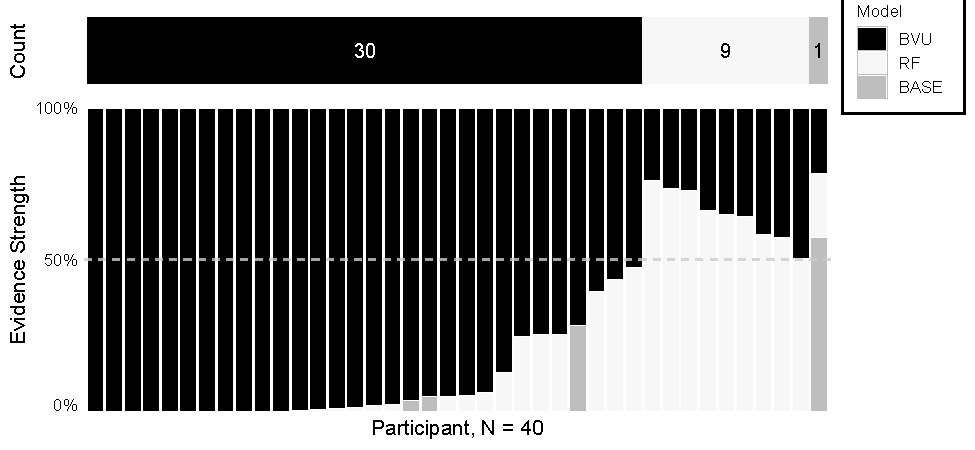
\includegraphics{../figures/study1_model_weights-1} 

}

\caption{Evidence for the models for individual participants. \textit{RF}$=$ relative frequency model, \textit{BVU}$=$ Bayesian value updating model, \textit{BASE}$=$ Baseline model.}\label{fig:study1_model_weights}
\end{figure}

\added[id=jj]{
The estimated parameter of the winning models, which Table \ref{tab:study1_parameter} summarizes, reveal that the power utility exponent ($\alpha$) is almost identical for the participants using a Bayesian value updating strategy ($M_{\alpha}= 1.43$) and those using a relative frequency strategy ($M_{\alpha}=1.60$), $M = -0.13$ 95\% HDI $[-0.71$, $0.38]$, $\mathrm{BF}_{\textrm{01}} = 3.26$. Participants using the Bayesian strategy had, on average, a prior belief that gains occur with 46\% (gain prior $\theta_G = 0.92$; zero-outcome prior $\theta_0 = 1.08$). Also, their estimated learning rate $\delta$ was anti-conservative ($M_{\delta}=1.36$; values $>$ 1 are liberal, 1 is optimal Bayesian, $<$ 1 is conservative learning); this contradicts previous results that found conservative learners \citep{Edwards1967,Tauber2017}, but the liberal learning in our task can be explained because participants repeatedly sampled from the same set of gambles.
}

\begin{table}[tbp]
\begin{center}
\begin{threeparttable}
\caption{\label{tab:study1_parameter}Parameter Estimates of Winning Models, \textit{M (SD)}}
\begin{tabular}{lccccc}
\toprule
Winning Model & $\alpha$ & $\delta$ & $\theta_G$ & $\mu$ & $\sigma$\\
\midrule
BVU (\textit{n}$=$30) & 1.49 (1.47) & 1.36 (2.12) & 0.92 (0.66) & -- & 0.13 (0.07)\\
RF (\textit{n}$=$9) & 1.61 (0.58) & -- & -- & -- & 0.12 (0.02)\\
BASE (\textit{n}$=$1) & -- & -- & -- & 0.47 (NA) & 0.30 (NA)\\
\bottomrule
\addlinespace
\end{tabular}
\begin{tablenotes}[para]
\normalsize{\textit{Note.} \textit{BVU}$=$ Bayesian value updating model, \textit{RF}$=$ relative frequency model, \textit{BASE}$=$baseline model. Parameters denote: $\alpha=$ power utility exponent, $\theta_G$ gain prior, $\mu=$ mean evaluation, $\sigma$ standard deviation.}
\end{tablenotes}
\end{threeparttable}
\end{center}
\end{table}

\textit{Qualitative Model Fit.}
\added[id=jj]{The qualitative fit between the models and the data is shown in Figure \ref{fig:ind_fits1}, which plots the predictions of the best-fitting models against the observed evaluations. It shows that the models generally describe the data well (mean $r\textsubscript{pred,obs} = 0.71$), except in four cases, where even the winning model fails to resemble the data qualitatively (participants number 05, 19, 24, 38, with $r\textsubscript{pred,obs} < 0.40$). For these cases, for whom the winning model is the Bayesian updating model, the model must be rejected because of qualitative mis-fit.}

\begin{figure}[htb]

{\centering 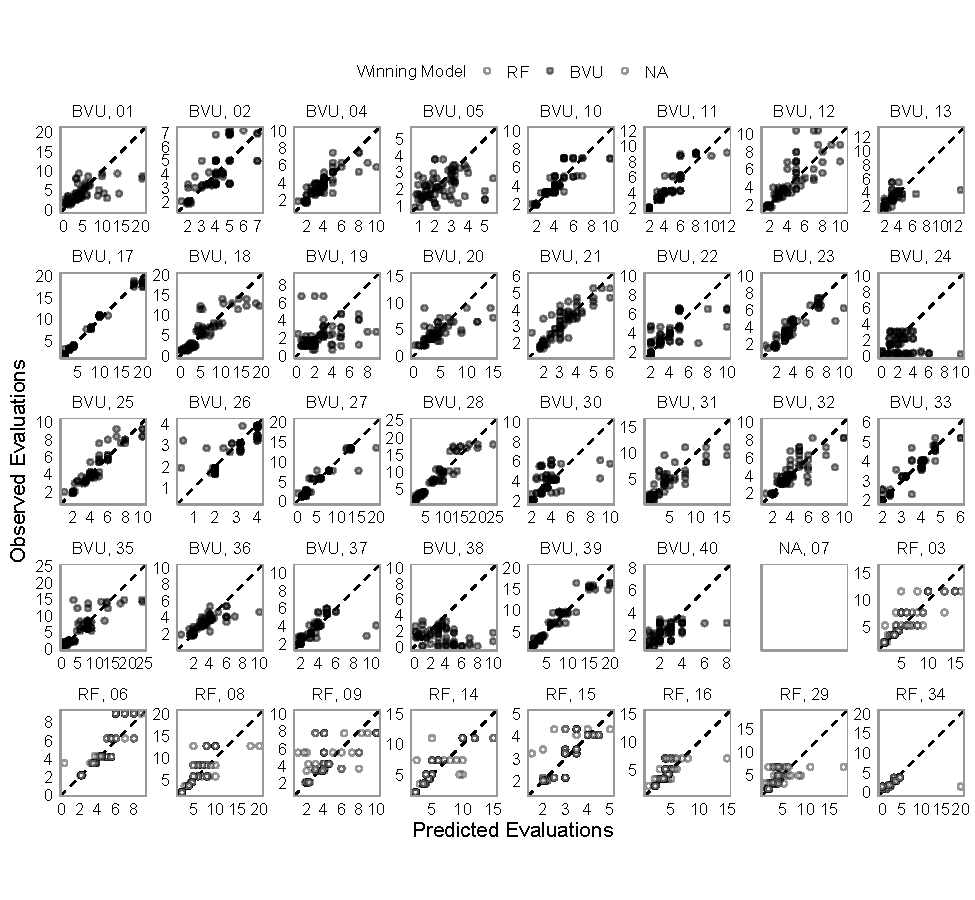
\includegraphics{../figures/ind_fits1-1} 

}

\caption{Predicted evaluations from the best-fitting models plotted against the observed evaluations (by participant). \textit{BVU}$=$ Bayesian value updating model, \textit{RF}$=$ relative frequency model, \textit{BASE}$=$baseline model.}\label{fig:ind_fits1}
\end{figure}

\added[id=jj]{The cognitive modeling results thus show that most participants used a Bayesian strategy, and some used a relative-frequency strategy. This strategy heterogeneity helps understanding the behavioral null finding---that sample size seemed to have no effect on valuations---that were observed at the aggregate level (Table \ref{tab:means_study1}). The aggregate analysis fails to take the individual differences in learning strategies into account, while participants are best described by a mixture of strategies. Moreover, the aggregate analysis also fails to account for differences in the prior beliefs about gain probabilities. Depending on the prior belief, the Bayesian value updating (BVU) model predicts either a decrease or an increase in valuations with increasing sample size. The next analysis will focus on these differences.}

\emph{The effect of sample size given cognitive strategies.} Next, we
qualitatively analyzed if sample size differentially affects the
relative-frequency-type and Bayesian-type learners. We expected that
sample size leads to changes in the evaluations of the Bayesian learners
depending on their priors, and that sample size does not affect the
evaluations of the relative-frequency learners. \added[id=jj]{
The Bayesian model predicts that sample size changes the evaluations differently as a function of prior beliefs. Participants with a gain prior---initially believing that gains are more likely than zero-outcomes---should decrease the evaluations of \$-bets as sample sizes increase, because participants overwrite their priors through sampling and learn that gains of \$-bets are less likely than zero-outcomes. By contrast, participants with a zero-outcome prior---initially believing that zero-outcomes are more likely than gains---should increase their evaluations of p-bets as sample size increases, because they learn that gains of p-bets are more likely than zero-outcomes (see the probabilities in Table~\ref{table:Lotteries}).
}

\textbackslash{}added{[}id=jj{]}\{ Based on the cognitive modeling
results, participants were classified into three learner types,
relative-frequency learners, Bayesian learners with gain priors (prior
\(\theta_G > 1\)), and Bayesian learners with loss priors (prior
\(\theta_G \leq 1\)). Figure \ref{fig:qual1} shows how the learner
types' evaluations of p-bets and \$-bets change with increasing sample
size. The relative-frequency learner types evaluated both p-bets and
\$-bets quite unaffected by sample sizes, whereas the Bayesian learner
types changed their evaluations slightly with sample size in the
predicted directions. Statistical analyses by means of a Bayesian
generalized linear
model\footnote{regressing the (normalized) evaluations on the predictors sample size, gamble type (p-bet, \$-bet), and type (BVU-gain-prior, BVU-loss-prior, RF) with a by-participant random intercept; categorical predictors were effects-coded to facilitate interpretation of interactions \citep[for details, see][]{SingmannForthcoming}), however, showed no substantial support that including the learner type as predictor improves goodness of fit, $BF\textsubscript{01}=0.393419762088619FALSE$, where 0 $=$ the model including learning type and 1 $=$ the model excluding learning type.
}

\begin{figure}[htb]

{\centering 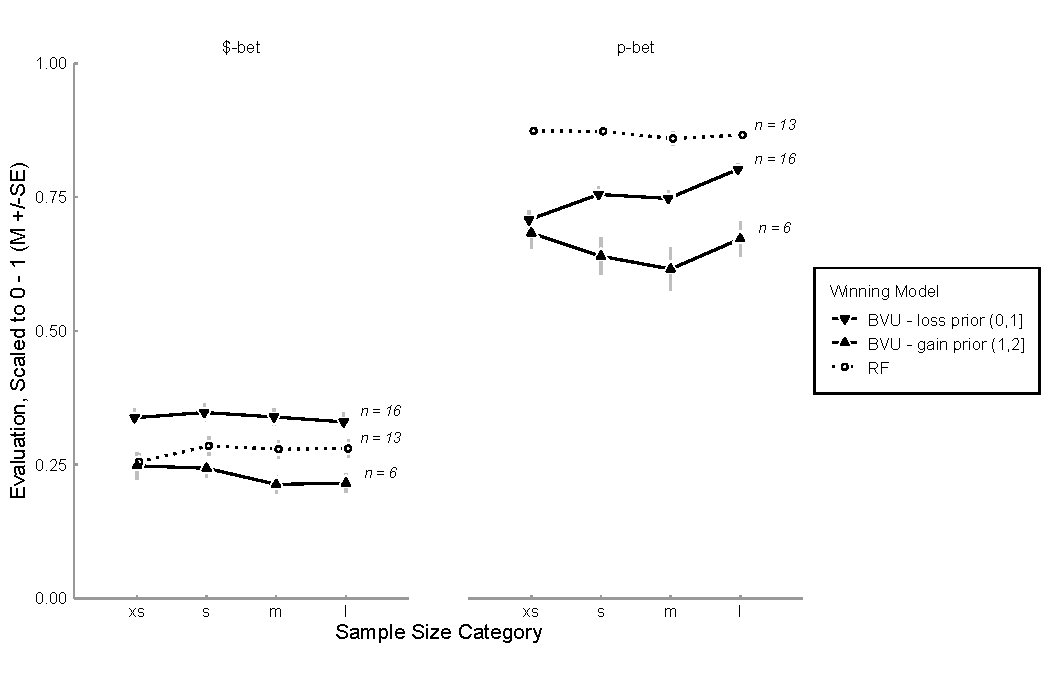
\includegraphics{../figures/qual1-1} 

}

\caption{Mean evaluation (standardized to 0 - 1) by winning model and prior beliefs of the BVU model. \textit{BVU}$=$Bayesian value updating model, \textit{RF}$=$ Relative frequency model. Error bars indicate standard errors. \textit{\$-bet}: low-probability high-outcome gambles, \textit{p-bet}: high-probability low-outcome gambles. Sample sizes (xs, x, m, l), see Table \ref{tab:Lotteries}. \textit{n=16, 13, 6} denotes the number of participants best-described by the respective models.}\label{fig:qual1}
\end{figure}

\subsubsection{Effect of gamble type and sampling order}

The mean and median evaluations of \$-bets were higher than for p-bets
(Gamble IDs 1--3 versus 4--6, Table \ref{tab:means_study1}), despite the
gambles having the same expected value. This finding is supported by
comparing a linear Bayesian regression model of gamble evaluations
\(\mathrm{M}\textsubscript{0}\)
\added[id=jj]{that includes the expected value as random effect} with a
model \(\mathrm{M}\textsubscript{1}\)
\added[id=jj]{that includes p-bets and \$-bets as fixed effects}
(\(BF\textsubscript{10} > 1,000\)).

To test for recency or primacy effects, we compared how well the first
half and the second half of the sample sequence in each trial predicts
valuations. A linear model \(\mathrm{M}\textsubscript{0}\) that predicts
valuations as a function of the random factor gamble ID outperforms a
model \(\mathrm{M}\textsubscript{1}\), which also includes the mean of
the first half of the observed samples as a fixed factor
(\(BF\textsubscript{01} = 16.6\)) and model
\(\mathrm{M}\textsubscript{2}\), which includes the mean of the second
half of observed samples (\(BF\textsubscript{02} = 6.7\)). In summary,
our analysis did not provide evidence for recency or primacy effects.

\subsubsection{Confidence ratings}

Participants' aggregated mean confidence ratings of their valuations
from experience in the extra small, small, medium, and large sample-size
categories were \(4.11\) (\(SD = 1.10\)), \(4.15\) (\(SD = 1.04\)),
\(4.14\) (\(SD = 1.03\)), and \(4.16\) (\(SD = 1.06\)) for xs, s, m, and
l (respectively). Sample size did not influence participants' confidence
systematically: \(\mathrm{M}\textsubscript{0}\), which predicts
confidence rating as a function of a random participant effect, was
strongly preferred over \(\mathrm{M}\textsubscript{1}\), which in
addition includes the sample-size category as a predictor
(\(BF\textsubscript{01} = 737\)).

\added[id=jj]{According to Bayesian value updating higher sample sizes should increase confidence. The relative frequency model predicts no influence of sample size on confidence. We analyzed the confidence ratings by best-fitting model (Bayesian-type learners and relative-frequency-type learners). The confidence of Bayesian learners did not change remarkably across sample sizes ($M=4.17, 4.09, 4.18, 4.17$ for sample sizes s, xs, l, m, respectively; $SD$s$=$ 0.99, 1.09, 1.02, 1.02, respectively). A linear model\footnote{with by-participant random intercept and the predictors effect-coded.} of the confidence ratings, which excluded sample size as predictor, was preferred over a model including sample size ($BF\textsubscript{excl,incl} = 3.01$).
  Similarly, the confidence of relative-frequency-type learners did not show an effect of sample size on confidence ratings ($M = 4.07, 4.14, 4.10, 4.10$ for sample sizes mxssl, respectively; \textit{SD}s$=$ 1.08, 1.17, 1.15, 1.20, respectively; BF\textsubscript{excl,incl}$= 0.00348182551069965FALSE$)}.

\subsubsection{Description versus experience}

The above Table \ref{tab:means_study1} shows the mean and median
valuations from description and the difference between the mean
valuations in the experience and description conditions. Further, it
provides the Bayes factors, quantifying the evidence in favor of a
difference between valuations from experience and those from
description.

Valuations made from description and experience differed for most of the
gambles and sample sizes (see Table \ref{table:meansStudy2}, rightmost
column). In particular, participants attached a higher value to
experienced than to described \$-bets (Gambles 1--3) but attached a
higher value to described than to experienced p-bets (Gambles 4--6).
Thus, we found a D--E gap that is the opposite of the classic D--E gap
observed in choice paradigms. In our study, participants valued gambles
as if they overweighted rare events from description \textit{and}
experience. This effect was even stronger when people made valuations
from experience.

We also compared participants' confidence ratings of valuations from
experience in each sample-size category to those from description
(\(M = 4.04\), \(SD = 1.08\)). Separately for each sample-size category,
we compared \(\mathrm{M}\textsubscript{0}\), which predicts confidence
as a function of random participant effects, with
\(\mathrm{M}\textsubscript{1}\), which takes condition as an additional
fixed factor into account. The analyses suggest that participants were
slightly more confident about their ratings from experience than from
description for small (\(BF\textsubscript{10} = 2.5\)), medium
(\(BF\textsubscript{10} = 1.3\)), and large
(\(BF\textsubscript{10} = 4.8\)) sample sizes. For the extra small
sample sizes (\(BF\textsubscript{10} = 0.3\)), confidence judgments did
not differ.


\end{document}


\subsubsection{Sample size}
%Table \ref{table:meansStudy2} displays the mean and median valuations from experience, that is, the monetary amount elicited with the BDM method, separately for each gamble and each sample-size category. The data suggest that sample size does not affect valuations from experience consistently. A model comparison supports this indication. Model $\mathrm{M}\textsubscript{0}$, which predicts valuations from experience as a function of the random factor expected value and the fixed factor gamble type (p-bet vs. \$-bet), is preferred over a model that takes into account sample size as an additional fixed factor ($BF\textsubscript{01} = 409$) and a model that additionally takes into account the interaction between sample size and gamble type ($BF\textsubscript{01} > 1,000$). 

% \begin{ThreePartTable}
% \begin{TableNotes}
% \small
% \item \textit{Note}. Median and mean valuations across participants. The heading $p$(gain) describes the probability $(p)$ with which a gain occurred and the gain amount in Swiss francs (gain). The probability is expressed as the ratio of the relative frequency of the number of gain observations to the number of observations in the smallest sample size category (xs) of this gamble. D--E describes the difference between mean valuations from description (D) and those from experience (E). Bayes factor $BF\textsubscript{10}$ quantifies the evidence for a linear model ($\mathrm{M}\textsubscript{1}$) that predicts that valuations differ between description and experience over a linear model ($\mathrm{M}\textsubscript{0}$) that predicts no such difference. Both models contain participant as a random factor. EV = expected value; xs = extra small; s = small; m = medium; l = large. Gambles 1, 2, and 3 represent \$-bets and Gambles 4, 5, and 6 represent p-bets.
% \end{TableNotes}
% \footnotesize
% \begin{longtable}{ccccccccc}
% \caption{Valuations, Study 1}\label{table:meansStudy2}\\
% \toprule
% Gamble & Condition & Sample size & \(p\)(gain) & EV& Median & Mean& D--E & $BF\textsubscript{10}$\\
% \midrule
% \multirow{5}{*}{1} &\multirow{4}{*}{E} & 5 (xs)  & \multirow{5}{*}{1/5(16.00)}& \multirow{5}{*}{3.20}
%  & 5.00 & 5.16 & 0.56 & 4.43\\
% && 10 (s) &&& 4.55 & 5.30& 0.70&64.94 \\
% && 15 (m)&&&5.00 & 5.34 & 0.74&24.12\\
% && 30 (l)&&& 5.00 & 5.29& 0.69&147.10\\
% & D &&&&  4.00 & 4.60 && \\
% \midrule
% \multirow{5}{*}{2} &\multirow{4}{*}{E} & 6 (xs)  & \multirow{5}{*}{1/6(12.00)}&  \multirow{5}{*}{2.00}
% & 4.00 & 4.33 & 0.72 &132.21\\
% && 12 (s) &&&   4.00 & 4.31 & 0.70&625.86 \\
% && 18 (m) &&&   4.00 & 4.04 & 0.43&4.46 \\
% && 36 (l) &&&   4.00 & 3.99 & 0.38 &1.85\\
% & D &&&&   3.00 & 3.61 && \\
% \midrule
% \multirow{5}{*}{3} &\multirow{4}{*}{E} & 7 (xs)  & \multirow{5}{*}{1/7(28.00)}& \multirow{5}{*}{4.03}
% & 6.00 & 7.56 & 0.99&4.32\\
% && 14 (s) &&& 6.70 & 8.40 & 1.83&905.21\\
% && 21 (m) &&&  6.20 & 7.92 & 1.35&141.95\\
% && 42 (l) &&& 6.00 & 7.68 & 1.11&15.99\\
% & D&&&&  5.00 & 6.57  &&\\
% \midrule
% \multirow{5}{*}{4} &\multirow{4}{*}{E} & 5 (xs)  & \multirow{5}{*}{4/5(4.00)}& \multirow{5}{*}{3.20}
% & 3.00 & 2.80 & -0.28&>1,000\\
% && 10 (s) &&& 3.20 & 2.92 & -0.16&3.24\\
% && 15 (m) &&&3.00 & 2.80 & -0.28&57.41\\
% && 30 (l) &&&3.00 & 2.95& -0.13&1.41\\
% & D &&&&  3.20 & 3.08 & &\\
% \midrule
% \multirow{5}{*}{5} &\multirow{4}{*}{E} & 6 (xs)  & \multirow{5}{*}{5/6(2.40)}&  \multirow{5}{*}{2.00} 
% & 2.00 & 1.77 & -0.10&8.03\\
% && 12 (s) &&&  2.00 & 1.75 & -0.12&14.56\\
% && 18 (m) &&&  2.00 & 1.73 & -0.14&28.34\\
% && 36 (l) &&&  2.00 & 1.81 & 0.06&0.71\\
% & D &&&&   2.00 & 1.87 && \\
% \midrule
% \multirow{5}{*}{6} &\multirow{4}{*}{E} & 7 (xs)  & \multirow{5}{*}{6/7(4.70)}& \multirow{5}{*}{4.03}
% & 4.00 & 3.46 & -0.18&2.66\\
% && 14 (s) &&&  4.00 & 3.55 & -0.09&0.34\\
% && 21 (m) &&&  4.00 & 3.58 & -0.06&0.19\\
% && 42 (l) &&&  4.00 & 3.70 & 0.06&0.22\\
% & D &&&&   4.00 & 3.64 & &\\
% \bottomrule
% \insertTableNotes
% \end{longtable}
% \end{ThreePartTable}


% der Unterschied zw. experience and description wird aber bei den meisten gambles mit einem grossen sample geringer. Könnte man noch erwähnen, müsste man nicht auf sig. testen, wäre aber auch möglich

\subsubsection{Modeling procedure}
To study the role of sample size more closely, we examined how well the RF model and the BVU model modeled participants' valuations in the experience condition. To test the psychological plausibility of both models, we also compared them to a baseline model. This baseline model predicts random responses, where each response between 0 and the gain amount is equally likely. 

Before estimation, we rescaled both the observed and the model-predicted valuations by dividing them by the possible gain of the gamble in a trial. Consequently, all data points lay in the interval between 0 and 1. All models were estimated by applying maximum likelihood methods to participants' individual data. To compute the likelihood, we assumed that observed valuations followed a truncated normal distribution around the model's predicted valuation with a standard deviation that was estimated as a free parameter for each participant. Thus, the RF and BVU models, but not the baseline model, were equipped with one additional free standard deviation parameter. We searched for the set of parameter values that minimized the deviance, defined as the negative log likelihood of the data given the model and its parameter values. To identify the best model parameters, we used a brute-force grid-search approach. We searched the parameter space for the utility parameter $\upalpha$ between $0$ and $3$ in steps of $0.025$ and for the standard deviation of the truncated normal distribution between $0.00001$ and $0.3$ in steps of $0.01$. We compared the models on Bayesian model weights that we computed from the Bayesian information criterion (\citealp{Kass1995, Lewandowsky2011}).

\subsubsection{Modeling results}
\begin{figure}[htbp] 
  \centering
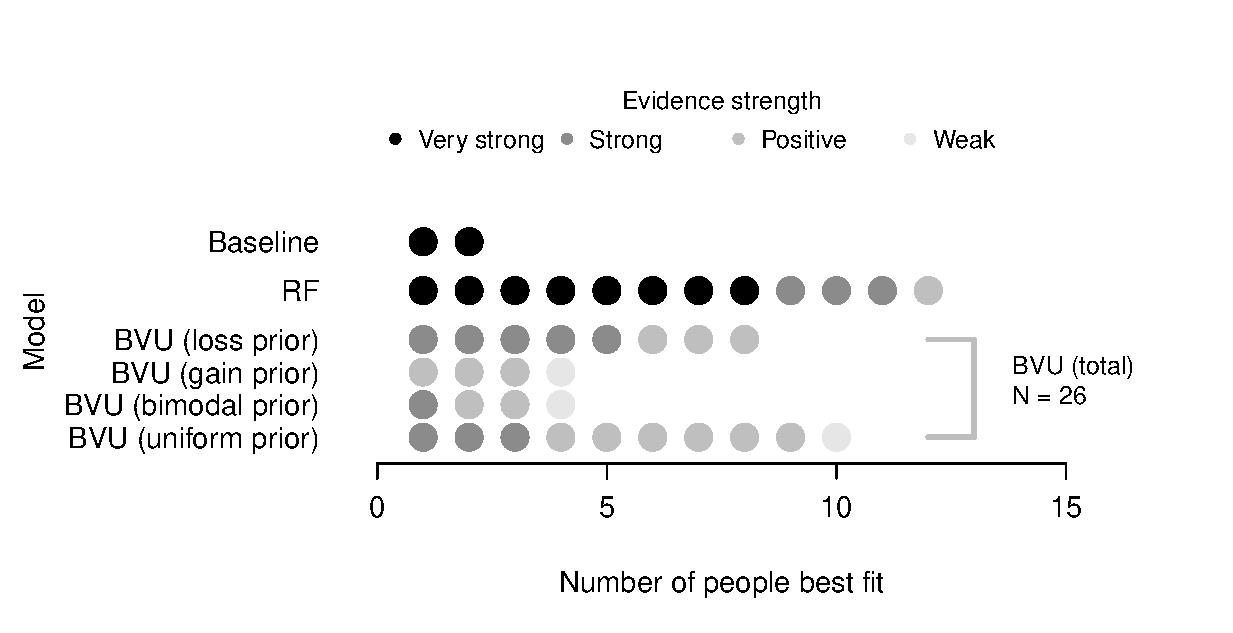
\includegraphics[width=.9\linewidth, keepaspectratio]{modelcomp_rs1.eps}
  \caption{Number of people who were best fit by each model. Evidence strength is indicated by shades of gray. Baseline = Baseline model; RF = relative frequency model; BVU = Bayesian value updating model \textcolor{blue}{ with the best fitting prior in parentheses.} }
  \label{fig:modeling1}
\end{figure}
Figure \ref{fig:modeling1} displays the relative evidence for each of the models. It shows for how many participants ($x$ axis) each model is favored and how strong this evidence is (grayscale). 

\textcolor{blue}{The data of 26 participants (65\%) were best described by the BVU model. Of these, 10 participants were best described with a uniform prior belief, 4 participants were best described with a bimodal prior belief, 4 participants were best described with a prior belief peaked over large gain probabilities (gain prior), and 8 participants were best described with a prior belief peaked over very low gain probabilities (loss prior). The evidence for individual participants is predominantly not very strong. An explanation for this finding is that for some trials, also a different prior belief could have described the data relatively well. If we only include the BVU model with the best fitting prior belief in the model comparison, the evidence strength is for 11 of the 26 participants very strong; for 6 of the 26 participants strong; for 6 of the 26 participants positive; and only for 3 of the 26 participants weak. For 12 participants (30\%), the RF model performed best. The data of 2 participants (5\%) were fit best by the baseline model.} 

\begin{figure}[htbp] 
  \centering
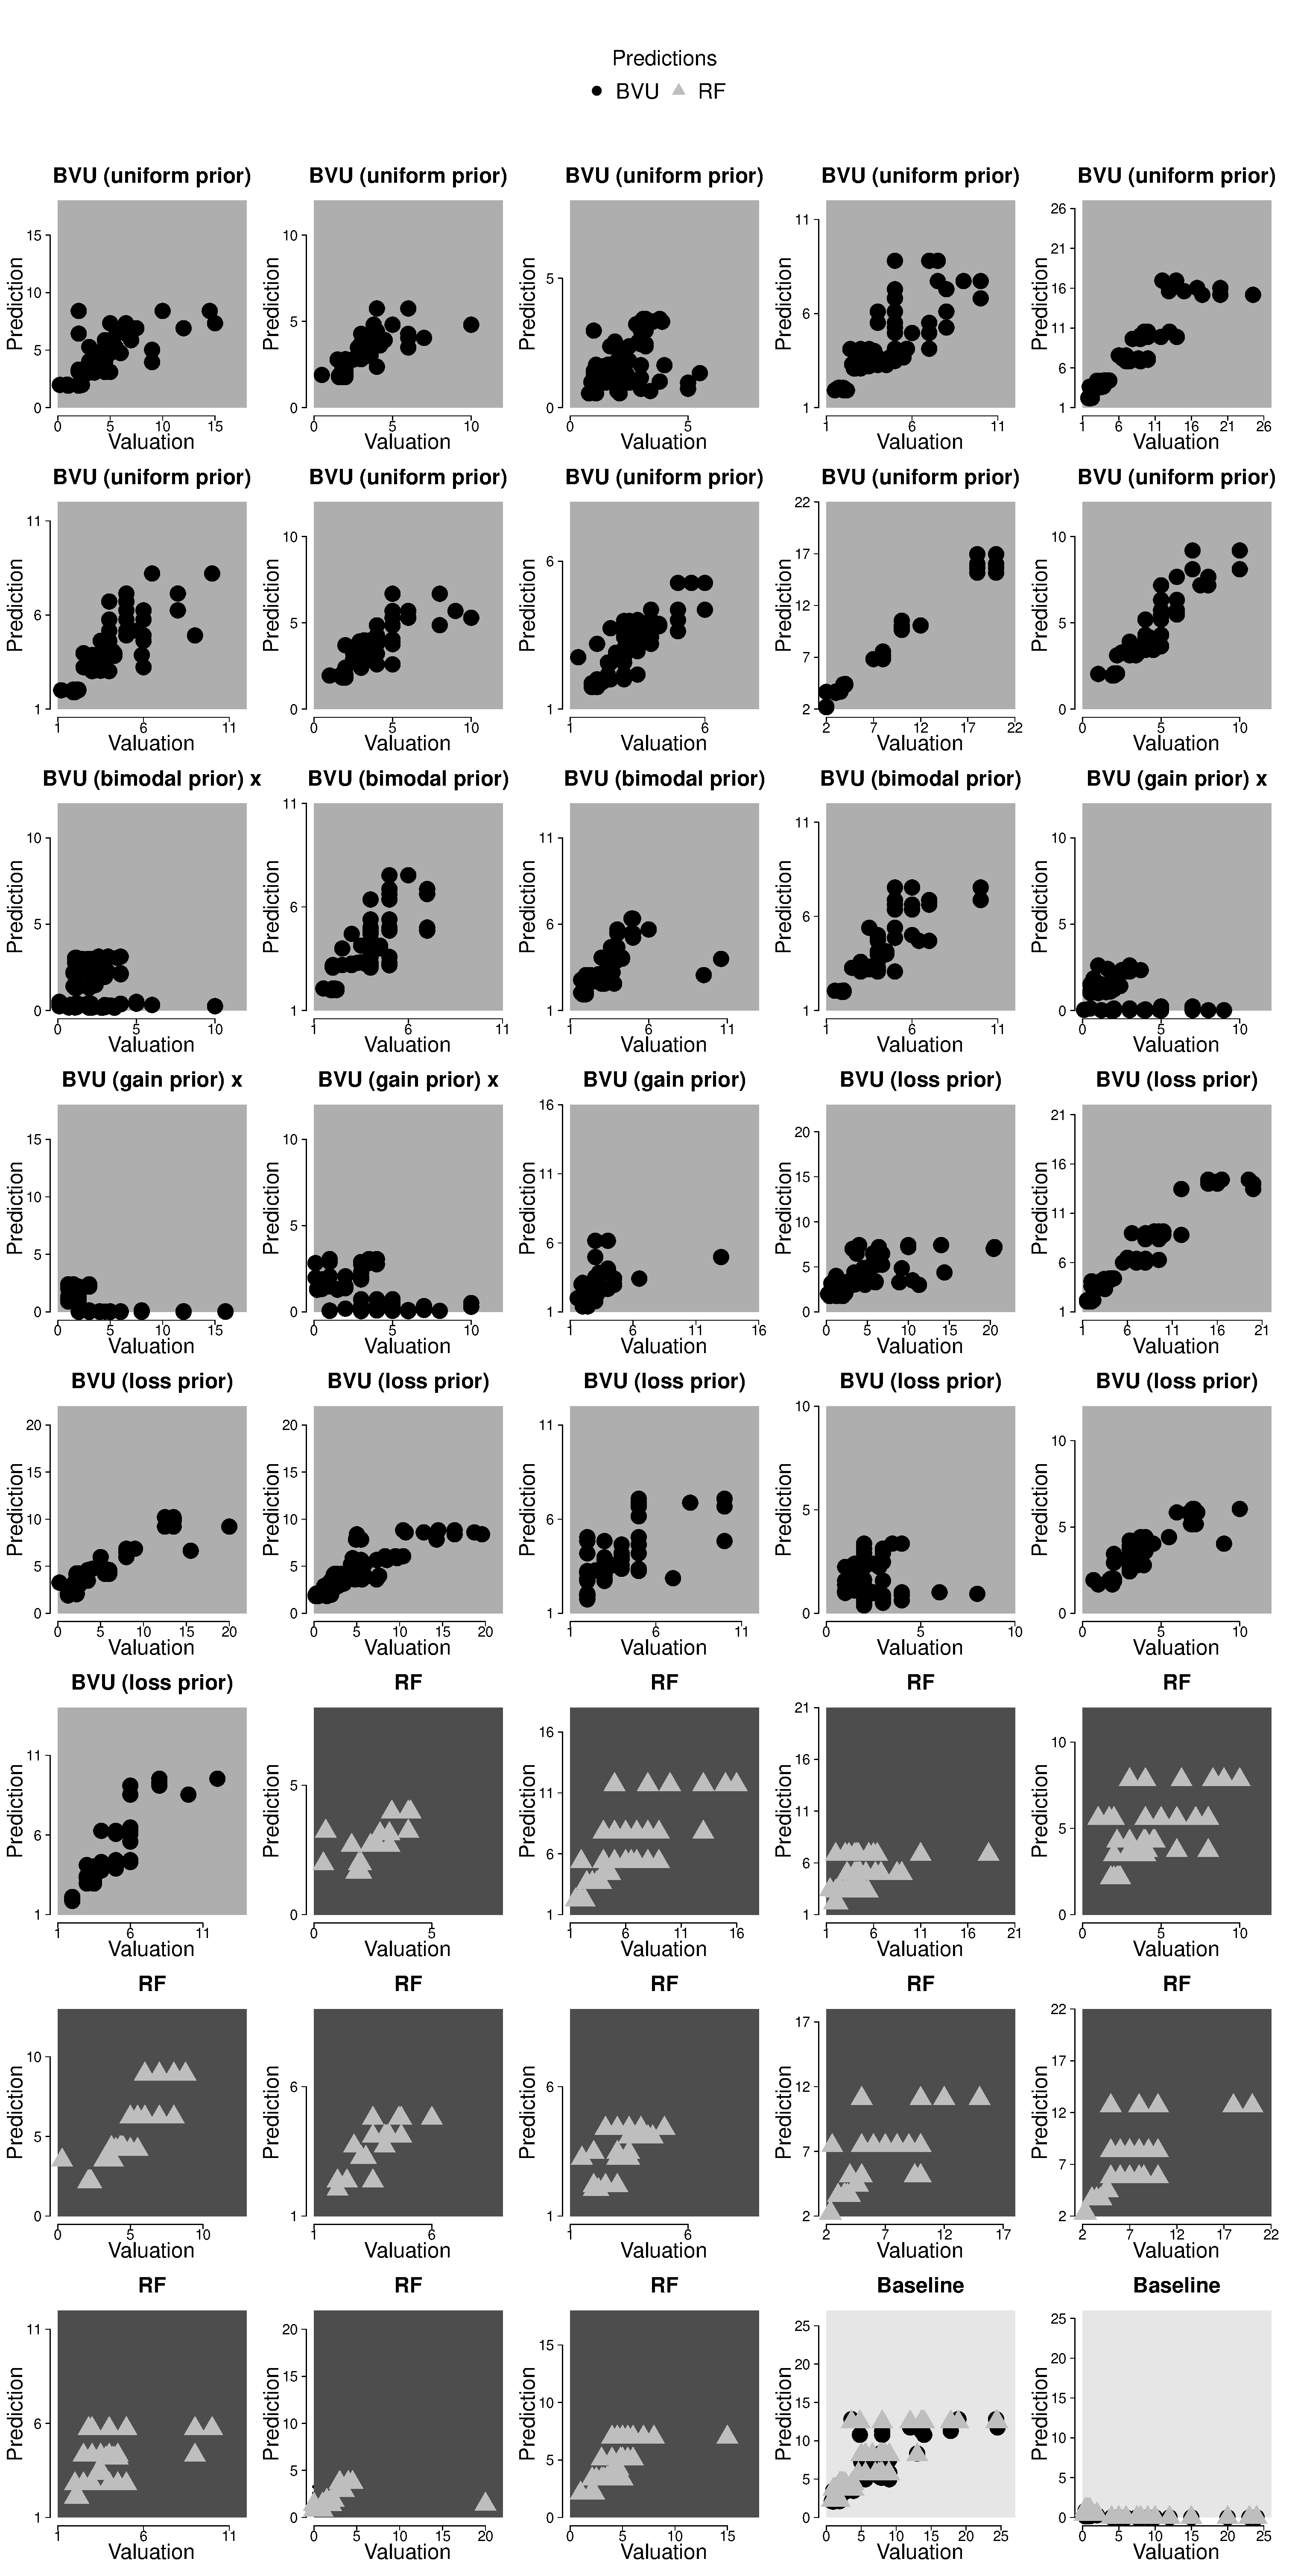
\includegraphics[height = .8\textheight, keepaspectratio]{indqual1.eps}%{ind_fits_study1.eps}
    \caption{Individual valuations plotted against model predictions given the optimal parameter estimates for each individual. The titles reflect the model that best fit the data and produced the predictions with the prior in parentheses. Participants for whom even the better fitting model qualitatively seem to not capture the data pattern well are marked with an x. BVU = Bayesian value updating; RF = relative frequency.}
  \label{fig:ind.fits1}
\end{figure}

Next, we explored the data using the results of the quantitative model comparison. For this purpose, we plotted individual valuations against the predictions made by the best fitting model separately for every participant given the optimal parameter estimates for that participant. This plot gives an indication of whether the models qualitatively capture data patterns. Figure \ref{fig:ind.fits1} shows that the models generally capture the data well. However, inspecting the figure reveals that in some cases, even the better fitting model does not capture the data patterns well. More precisely, this holds for four participants (marked with an x in Figure \ref{fig:ind.fits1}). For these participants the model is rejected because of the lack of qualitative fit.

\textcolor{blue}{Two reasons can explain why we did not find an effect of sample size on gamble valuations, as we observed in the previous analysis on the aggregate data. First, some participants were best described by the BVU model (Bayesian learners) and some participants by the RF model (frequentist learners). Yet, only Bayesian learners are expected to attend to sample size. Second, depending on the prior belief, the BVU model predicts either a decrease or an increase in valuations with growing sample size.}


Therefore, we next qualitatively investigated how the valuations of frequentist and Bayesian learners differ. We expected an effect of sample size only for Bayesian and not for frequentist learners. \textcolor{blue}{Separately for \$-bets and p-bets, we split Bayesian learners into two groups: For \$-bets, in one group we put those people who were best described by a model with a uniform prior, a bimodal prior, or a prior peaked over high gain probabilities. For these people, we expected a decrease in valuations with growing sample size. In the second group, we put those people who were best described by a model with a prior peaked over low gain probabilities. For these people, we expected an increase in valuations with growing sample size. For p-bets, in one group we put people who were best described by a model with a uniform prior, a bimodal prior, or a prior peaked over low gain probabilities. For these people, we expected an increase in valuations with growing sample size. In the second group, we put those people who were best described with a prior peaked over high gain probabilities. For these people, we expected a decrease in valuations with growing sample size.}  
Figure \ref{fig:qual1} shows the mean ratings for \$-bets and p-bets separately for participants quantitatively and qualitatively best described by either the BVU \textcolor{blue}{split into two groups as described above} or the RF model. The figure shows that the mean valuations of Bayesian learners indeed differed from the mean valuations of frequentist learners: The mean valuations of Bayesian learners \textcolor{blue}{changed as a function of sample size for both \$-bets and p-bets. Depending on whether the model suggested an increase or a decrease in valuations, people's valuations increased or decreased.
Yet, when we further statistically investigated this result only the increase in valuations of Bayesian learners for p-bets was reliable ($BF\textsubscript{10} > 1,000$, both $BF\textsubscript{10} < 1$ for \$-bets). Admittedly, the lack of statistical support for changes in valuations for Bayesian learners and \$-bets may have been the result of splitting Bayesian learners into two groups depending on whether the model predicts an increase or a decrease in valuations. For \$-bets, this procedure leads to a small \textit{N} (increasing = 8 and decreasing = 14) and hence very low statistical power. The mean valuations of frequentist learners did not show consistent variation (both gamble types $BF\textsubscript{10} < 1$).}



\begin{figure}[htbp] 
  \centering
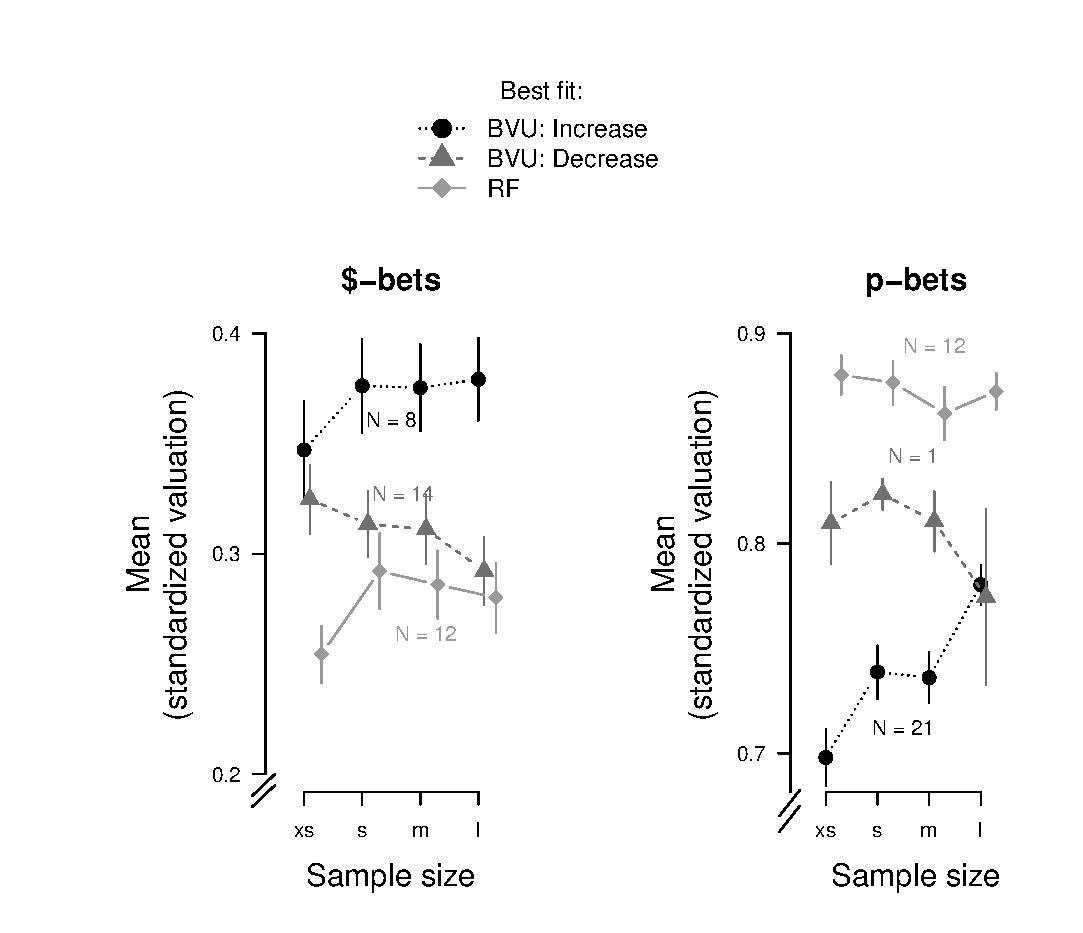
\includegraphics[width=.8\linewidth, keepaspectratio]{groupqual1_stand.eps}
  \caption{\textcolor{blue}{Mean valuations (standardized per gamble between 0 and 1) of participants who were best described by the Bayesian value updating (BVU) model (black and dark gray) and the relative frequency (RF) model (light gray).  Depending on whether the BVU model predicted an increase (black) or a decrease (dark gray) in valuations with growing sample size, separately for \$-bets and p-bets we split Bayesian learners into two groups (Increase and Decrease). $N$ describes on how many people's data the means are based. 
   Error bars indicate the standard error of the mean. Sample sizes: xs = extra small; s = small; m = medium; l = large.}}
  \label{fig:qual1}
\end{figure}

\subsubsection{Effect of gamble type and sampling order}
The mean and median ratings in Table \ref{table:meansStudy2} show that valuations for \$-bets (Gambles 1--3) were higher than for p-bets (Gambles 4--6), even if the gambles had the same expected value. This finding is supported by comparing model $\mathrm{M}\textsubscript{0}$, which assumes that gamble valuation can be predicted as a function of the random factor expected value, and model $\mathrm{M}\textsubscript{1}$, which makes the additional assumption that valuations differ between p-bets and \$-bets ($BF\textsubscript{10} > 1,000$).

To test also for recency or primacy effects, we compared how well the first half and the second half of the sample sequence in each trial predicts valuations. A linear model $\mathrm{M}\textsubscript{0}$ that predicts valuations as a function of the random factor gamble (1--6) outperforms model $\mathrm{M}\textsubscript{1}$, which also includes the mean of the first half of the observed samples as a fixed factor ($BF\textsubscript{01} = 16.6$) and model $\mathrm{M}\textsubscript{2}$, which includes the mean of the second half of observed samples ($BF\textsubscript{02} = 6.7$). In summary, our analysis did not provide evidence for recency or primacy effects.

\subsubsection{Confidence ratings}
Participants' mean confidence ratings of their valuations from experience in the extra small, small, medium, and large sample-size categories were xs = $4.11$ ($SD = 1.10$); s = $4.15$ ($SD = 1.04$); m = $4.14$ ($SD = 1.03$); and l = $4.16$ ($SD = 1.06$). Sample size did not influence participants' confidence systematically: $\mathrm{M}\textsubscript{0}$, which predicts confidence rating as a function of a random participant effect, was strongly preferred over $\mathrm{M}\textsubscript{1}$, which in addition includes the sample-size category as a predictor ($BF\textsubscript{01} = 737$).

Because only the BVU model predicts increasing confidence ratings as a function of sample size, we repeated the previous analysis separately for Bayesian and frequentist learners.
\textcolor{blue}{When considering only those data sets that were best described by the BVU model, confidence was lowest for extra small sample sizes (mean confidence ratings: xs = $3.90$, $SD = 1.03$; s = $4.06$, $SD = 0.91$; m = $4.04$, $SD = 0.93$; l = $4.06$, $SD = 0.97$). However, the simpler model that predicts no influence of sample size was slightly preferred over the model that predicts an effect of sample size ($BF\textsubscript{01} = 3.1$).}
%OLD:(mean confidence ratings: xs = $3.87$, $SD = 1.05$; s = $4.05$, $SD = 0.94$; m = $4.03$, $SD = 0.94$; l = $4.09$, $SD = 0.96$; $BF\textsubscript{10} = 2.94$). 
The analysis of those participants who were quantitatively and qualitatively best described by the RF model \textcolor{blue}{also} did not show an effect of sample size on confidence ratings \textcolor{blue}{(mean confidence ratings: xs = $4.45$, $SD = 1.22$; s = $4.37$, $SD = 1.2$; m = $4.35$, $SD = 1.17$; l = $4.35$, $SD = 1.21$; $BF\textsubscript{01} = 108$)}.


\subsubsection{Description versus experience}
Table \ref{table:meansStudy2} displays the mean and median valuations from description. It also shows the difference between the mean valuations in the experience and description conditions (column D--E, separately for different sample sizes). Further, it provides the Bayes factors, quantifying the evidence in favor of a difference between valuations from experience and those from description.

%\begin{center} --- Insert Table \ref{table:meansStudy2} here ---- \end{center}

Valuations made from description and experience differed for most of the gambles and sample sizes (see Table \ref{table:meansStudy2}, rightmost column). In particular, participants attached a higher value to experienced than to described \$-bets (Gambles 1--3) but attached a higher value to described than to experienced p-bets (Gambles 4--6). Thus, we found a D--E gap that is the opposite of the classic D--E gap observed in choice paradigms. In our study, participants valued gambles as if they overweighted rare events from description \textit{and} experience. This effect was even stronger when people made valuations from experience.

We also compared participants' confidence ratings of valuations from experience in each sample-size category to those from description ($M = 4.04$, $SD = 1.08$). Separately for each sample-size category, we compared $\mathrm{M}\textsubscript{0}$, which predicts confidence as a function of random participant effects, with $\mathrm{M}\textsubscript{1}$, which takes condition as an additional fixed factor into account. The analyses suggest that participants were slightly more confident about their ratings from experience than from description for small ($BF\textsubscript{10} = 2.5$), medium ($BF\textsubscript{10} = 1.3$), and large ($BF\textsubscript{10} = 4.8$) sample sizes. For the extra small sample sizes ($BF\textsubscript{10} = 0.3$), confidence judgments did not differ. 


\subsection{Discussion of Study 1}

Study 1 shows that the size of the sample overall did not have an effect on valuations from experience. However, our quantitative model comparison shows that roughly half of the participants were best described by a BVU model that assumes that people treat sample size as a measure of uncertainty. The other half of participants were best described by the RF model that disregards sample size. These results explain why we failed to find an effect of sample size across the whole data set. 

Qualitatively, the valuations of people best described by the RF model differed from those of people best described by the BVU model. Figure \ref{fig:qual1} illustrates the trend that valuations of people best described by the BVU model changed as a function of sample size. Especially for p-bets, valuations increased as sample size grew. % The BVU model assumes that people start sampling with the prior belief that all gain probabilities are equally likely. Through sampling, people update their probability belief. The more samples people observe, the more their gain-probability gets shifted from 50\% towards the true gain probability which implies with sample size increasing valuations for p-bets and decreasing valuations for \$-bets. 
For participants best described by the RF model, valuations appear not to have varied systematically with sample size. 

Valuations also differed when made from description versus experience. Interestingly, this difference is the opposite of the classic D--E gap that has been reported in choice paradigms: We found evidence that people behaved as if they overweighted rare events when making valuations from description \textit{and} experience. Notably, this overweighting of rare events was even stronger for the experience condition. Importantly, people assigned higher valuations to \$-bets (i.e., gambles that provide a high reward with low probability) than p-bets (i.e., gambles that provide a small reward with low probability) even when both gambles had similar expected values. This finding is in line with recent research that suggested people overweight extreme outcomes in experience-based tasks \citep{Ludvig2017}.

We found that participants' confidence in their valuations was generally high ($M = 4.12$, $SD = 1.06$ on a scale of 0 to 6). Importantly, only when we restricted the analysis to participants who were best described as Bayesian learners did we find that confidence increased with sample size as predicted by Bayesian models. We did not find an effect of sample size for participants who were best described by the RF model. If there was any trend, it seemed that confidence decreased with growing sample size, in line with \cite{Griffin1992}. Further, we found evidence that people were more confident in their valuations from experience than from description. 


\section{Study 2}
In Study 1, participants knew the outcomes before they started sampling. This is different from typical studies on decisions from experience, in which people have to learn the value of the outcomes during the sampling process. Therefore, \textcolor{blue}{to bring our method more in line with that of other studies}, in Study 2 we changed our experimental method such that the outcomes were learned from sampling.
\subsection{Method and Results}
Before participants started sampling, they knew only that each gamble consisted of two outcomes, of which one was 0 and the other a gain. In contrast to Study 1, the precise gain amounts were not displayed above the virtual urn before or during the sampling stage. In all other aspects, Study 2 was identical to Study 1. 

Forty people (38 women, 2 men) between 18 and 27 years old ($M = 21.1$ years, $SD = 2.05$) from the subject pool of the University of Basel participated. We followed the incentive scheme of Study 1. On average, participants earned a bonus of 7.16 CHF ($SD = 6.91$). For the data analysis, we compared the same statistical models as described in Study 1.

\begin{ThreePartTable}
\begin{TableNotes}
\small
\item \textit{Note}. Median and mean valuations across participants. The heading $p$(gain) describes the probability $(p)$ with which a gain occurred and the gain amount in Swiss francs (gain). The probability is expressed as the ratio of the relative frequency of the number of gain observations to the number of observations in the smallest sample size category (xs) of this gamble. D--E describes the difference between mean valuations from description (D) and those from experience (E). Bayes factor BF\textsubscript{10} quantifies the evidence for a linear model ($\mathrm{M}\textsubscript{1}$) that predicts that valuations differ between description and experience over a linear model ($\mathrm{M}\textsubscript{0}$) that predicts no such difference. Both models contain participant as a random factor. EV = expected value; xs = extra small; s = small; m = medium; l = large. Gambles 1, 2, and 3 represent \$-bets and Gambles 4, 5, and 6 represent p-bets.
\end{TableNotes}
\footnotesize
\begin{longtable}{ccccccccc}
\caption{Valuations, Study 2}\label{table:meansStudy3}\\
\toprule
Gamble & Condition & Sample size & \(p\)(gain) &  EV& Median & Mean& D--E& $BF\textsubscript{10}$\\
\hline
\multirow{5}{*}{1} &\multirow{4}{*}{Experience} & 5 (xs)  & \multirow{5}{*}{1/5(16)}& \multirow{5}{*}{3.20}
 & 5.15 & 6.29 & 0.86&11.13\\
&& 10 (s) &&& 5.00 & 6.39 & 0.96& 354.66\\
&& 15 (m)&&&5.95 & 6.38 & 0.95&78.07\\
&& 30 (l)&&& 6.00 & 6.53 & 1.10&171.43\\
& Description &&&&  4.00 & 5.43 && \\
\hline
\multirow{5}{*}{2} &\multirow{4}{*}{Experience} & 6 (xs)  & \multirow{5}{*}{1/6(12)}& \multirow{5}{*}{2.00}
& 4.00 & 4.55 & 0.24&0.26 \\
&& 12 (s) &&&   4.00 & 4.72 & 0.41&1.25 \\
&& 18 (m) &&&   5.00 & 4.88 & 0.57 &3.99\\
&& 36 (l) &&&   4.95 & 4.78 & 0.47 &3.58\\
& Description &&&&   3.35 & 4.31 && \\
\hline
\multirow{5}{*}{3} &\multirow{4}{*}{Experience} & 7 (xs)  & \multirow{5}{*}{1/7(28)}&  \multirow{5}{*}{4.03}
& 8.95 & 10.66 & 1.40&5.80\\
&& 14 (s) &&& 10.00 & 10.26 & 1.01&1.04\\
&& 21 (m) &&&  9.70 & 10.37 & 1.12&1.67\\
&& 42 (l) &&& 10.00 & 11.18 & 1.93&220.94\\
& Description&&&&  6.00 & 9.25  &&\\
\hline
\multirow{5}{*}{4} &\multirow{4}{*}{Experience} & 5 (xs)  & \multirow{5}{*}{4/5(4)}&  \multirow{5}{*}{3.20}
& 3.30 & 2.91 & -0.29&13.53\\
&& 10 (s) &&& 3.20 & 2.94 & -0.26&25.50\\
&& 15 (m) &&&3.20 & 3.02 & -0.18&1.74\\
&& 30 (l) &&&3.20 & 3.09 & -0.11&0.42\\
& Description &&&&  3.50 & 3.20 && \\
\hline
\multirow{5}{*}{5} &\multirow{4}{*}{Experience} & 6 (xs)  & \multirow{5}{*}{5/6(2.4)} & \multirow{5}{*}{2.00}
& 2.00 & 1.82 & -0.10&1.32\\
&& 12 (s) &&&  2.00 & 1.85 & -0.07&0.37\\
&& 18 (m) &&&  2.00 & 1.85 & -0.07&0.34\\
&& 36 (l) &&&  2.10 & 1.95 & 0.03&0.20\\
& Description &&&&   2.00 & 1.92 && \\
\hline
\multirow{5}{*}{6} &\multirow{4}{*}{Experience} & 7 (xs)  & \multirow{5}{*}{6/7(4.7)}& \multirow{5}{*}{4.03}
& 4.00 & 3.68 & -0.16&0.60\\
&& 14 (s) &&&  4.10 & 3.78 & -0.06&0.17\\
&& 21 (m) &&&  4.15 & 3.85 & 0.01&0.14\\
&& 42 (l) &&&  4.20 & 3.90 & 0.06&0.18\\
& Description &&&&   4.10 & 3.84 && \\
\bottomrule
\insertTableNotes
\end{longtable}
\end{ThreePartTable}
%\end{table*}


%\begin{center} --- Insert Table \ref{table:meansStudy3} here ---- \end{center}

\subsubsection{Sample size}
Table \ref{table:meansStudy3} displays mean and median valuations per gamble and sample-size category. Similar to in Study 1, mean valuations did not differ much between sample sizes: Again, valuations were best predicted by the random factor expected value and the fixed factor gamble type (additional fixed factor sample size: $BF\textsubscript{01} = 285$; additional interaction between sample size and gamble type: $BF\textsubscript{01} > 1,000 $). 

\subsubsection{Modeling results}

\begin{figure}[htbp] 
  \centering
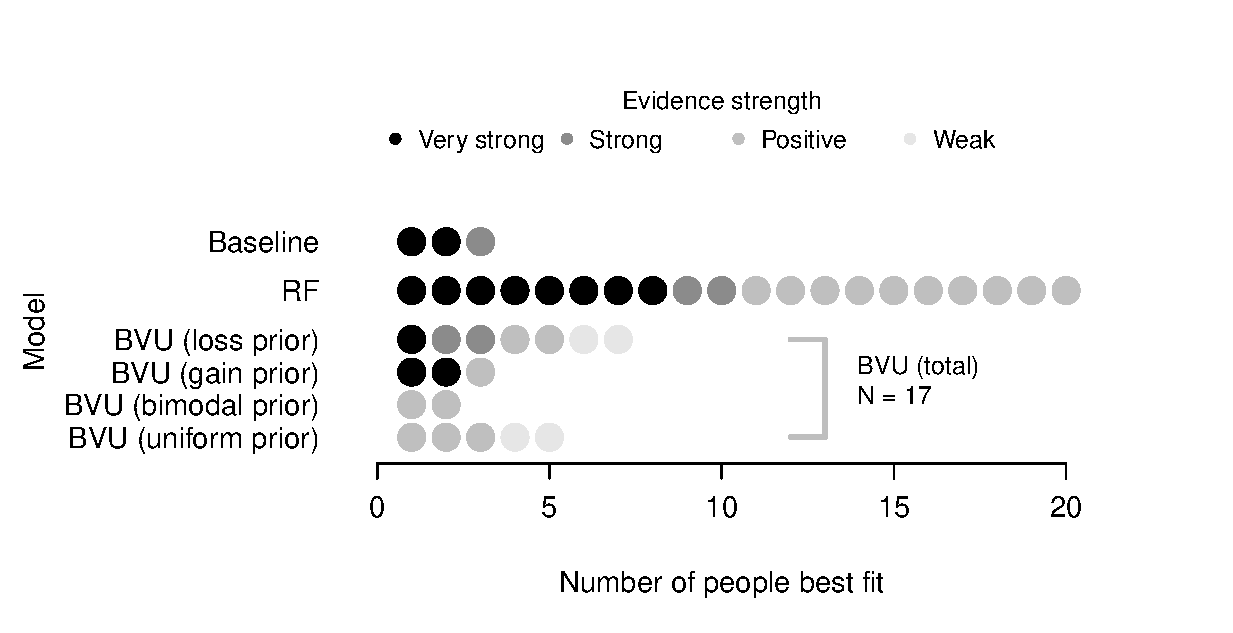
\includegraphics[width=.8\linewidth, keepaspectratio]{modelcomp_rs2.eps}
  \caption{Number of people who were best fit by each model. Evidence strength is indicated by shades of gray. Baseline = Baseline model; RF = relative frequency model; BVU = Bayesian value updating model \textcolor{blue}{ (with the best fitting priors in parentheses).} }
  \label{fig:modeling2}
\end{figure}

\textcolor{blue}{For the majority of participants (20 people, 50\% of all participants), the RF  model performed best. The behavior of 17 participants (42.5\%) was best described by the BVU model. Of these, 5 participants were best described with a uniform prior belief, 2 participants were best described with a bimodal prior belief, 3 participants were best described with a prior belief peaked over large gain probabilities (gain prior), and 7 participants were best described with a prior belief peaked over very low gain probabilities (loss prior). Again, if we included only the BVU model with the best fitting prior belief in the model comparison, the evidence is for 6 of the 17 participants very strong; for 2 of the 17 participants strong; for 7 of the 17 participants positive; and for only 2 of the 17 participants weak.  The baseline model was preferred for 3 participants (7.5\%). Generally, the results illustrate the psychological plausibility of both models, but the dominance of the RF model shows that most participants were not very sensitive to the sample sizes.} 


\begin{figure}[htbp] 
  \centering
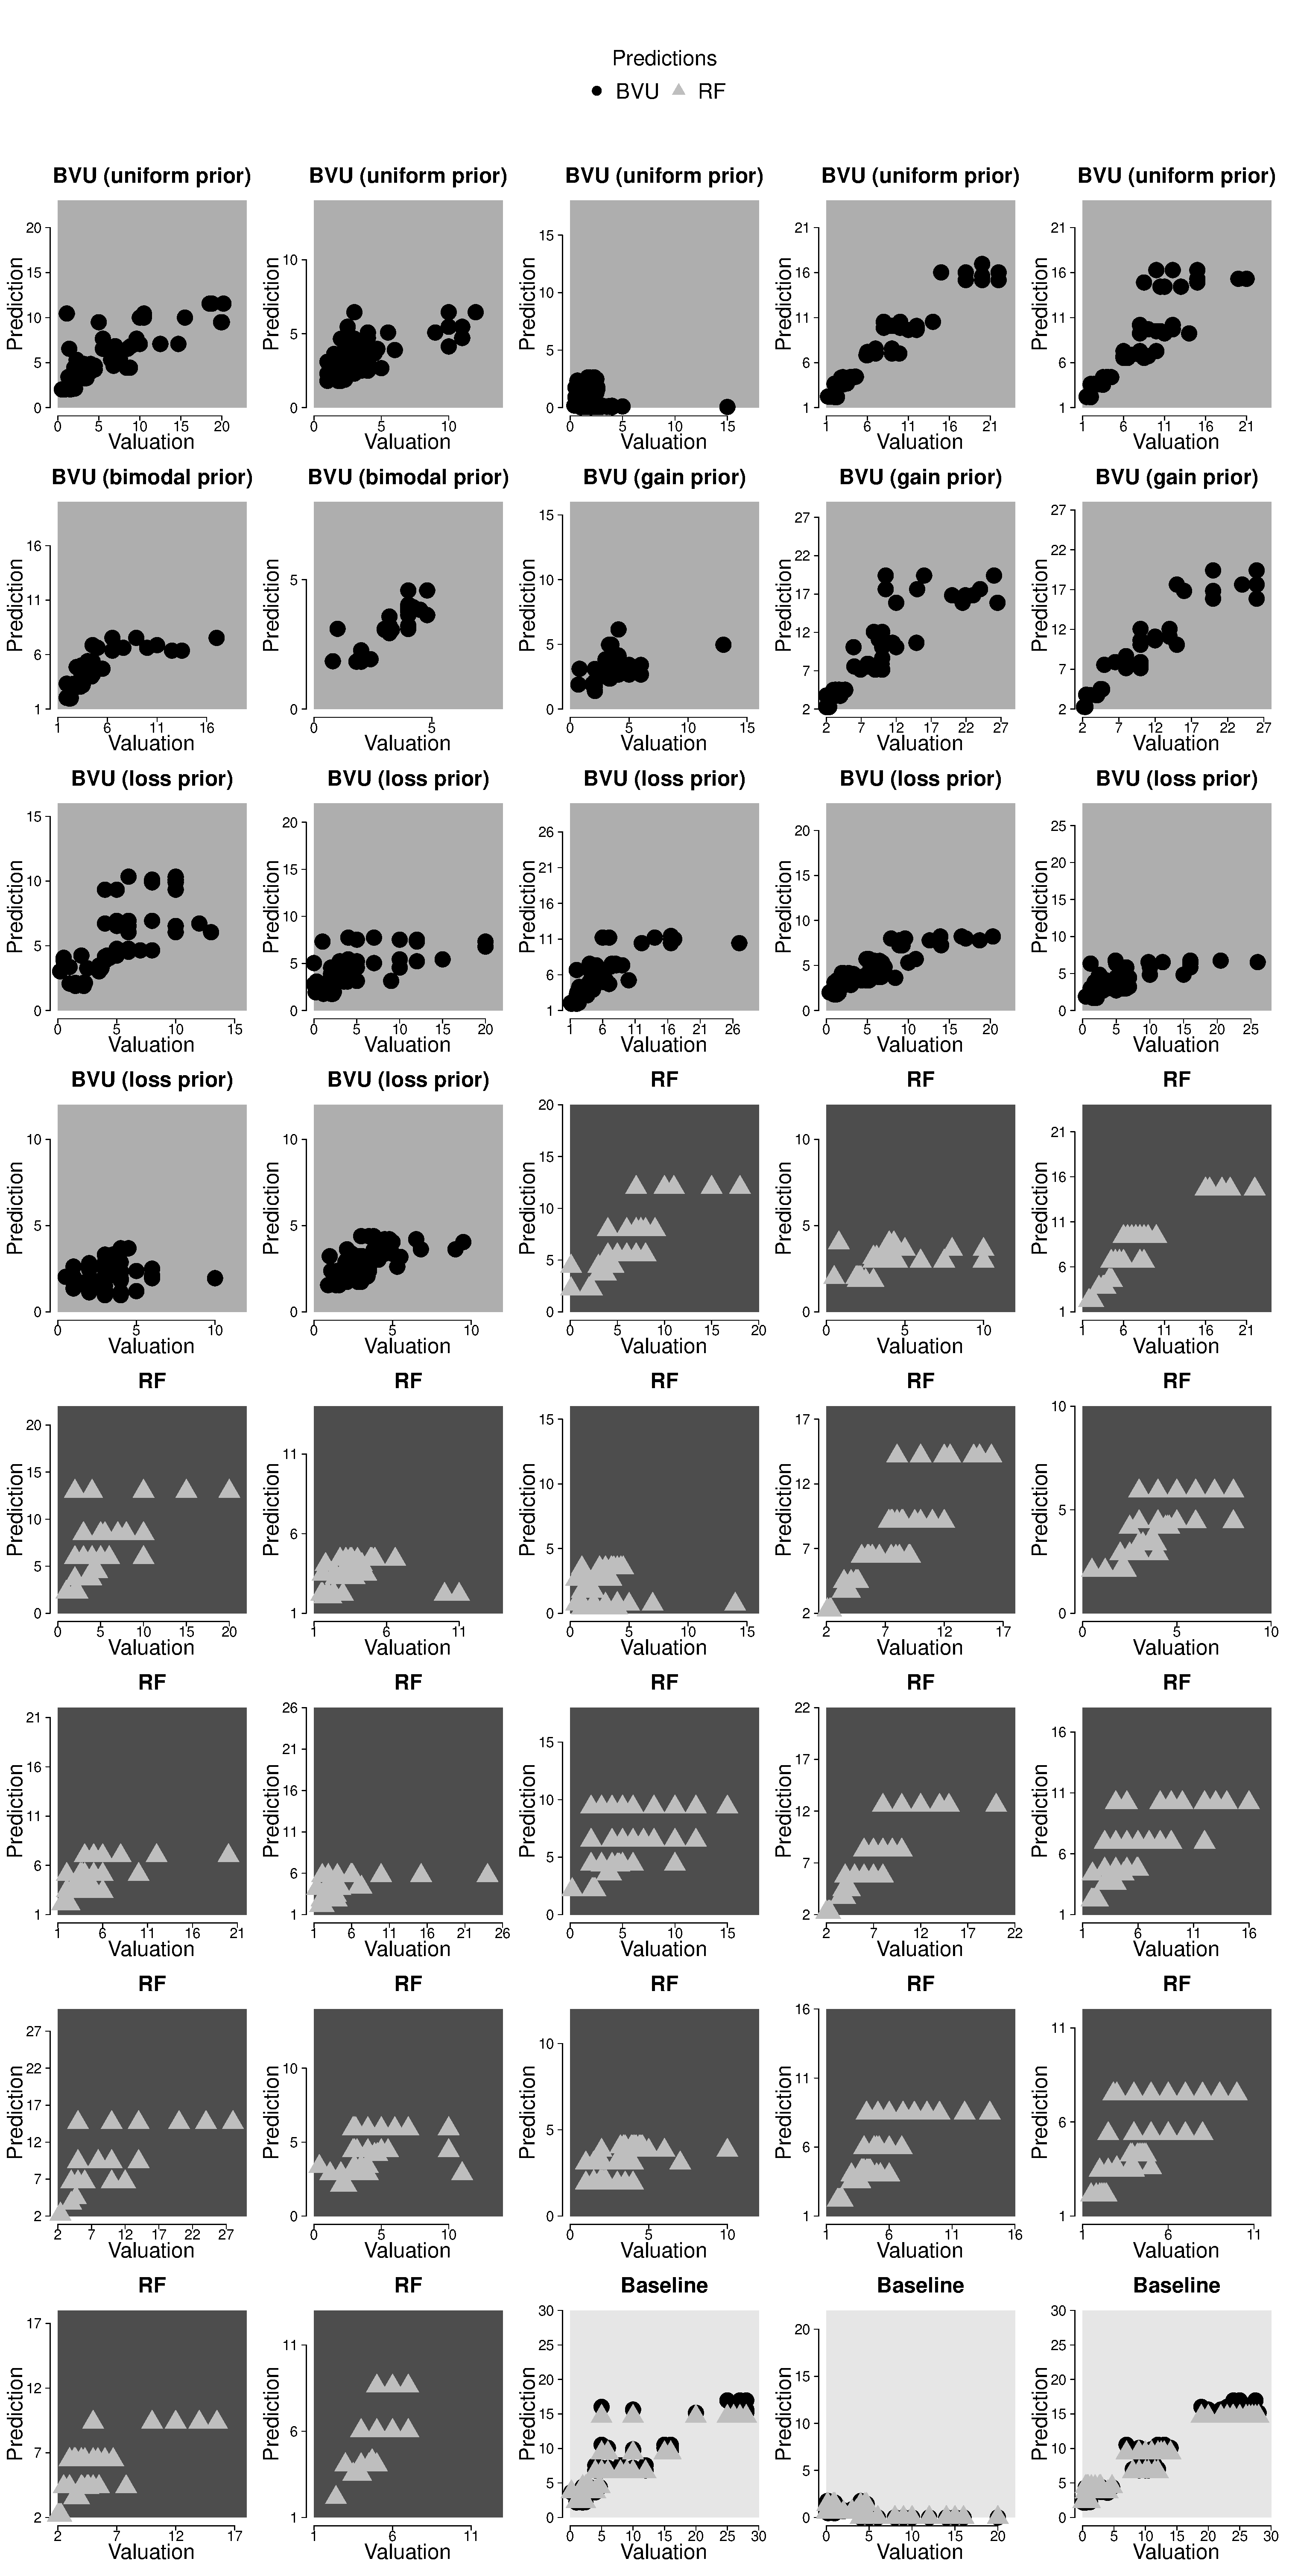
\includegraphics[height = .8\textheight, keepaspectratio]{indqual2.eps}
  \caption{Individual valuations plotted against model predictions given the optimal parameter estimates for each individual. The headings reflect the model that best fit the data and produced the predictions. BVU = Bayesian value updating (with the best fitting priors in parentheses); RF = relative frequency.}
  \label{fig:ind.fits2}
\end{figure}

As in Study 1, we examined the data qualitatively. In Figure \ref{fig:ind.fits2}, participants' valuations are plotted against the predicted valuations of the best fitting model given the optimal parameter estimates for each individual. Again the predictions capture the data well. Figure \ref{fig:qual2} shows the mean valuations of the frequentist and Bayesian learners separately for \$-bets and p-bets. Again, the two groups differed. 
\textcolor{blue}{For \$-bets, valuations of frequentist learners seem on average to slightly increase with growing sample size. This observation contrasts with the model predictions yet is statistically not reliable ($BF\textsubscript{01} = 1.5$).  As expected, for p-bets, average valuations of frequentist learners remain stable ($BF\textsubscript{01} = 89$). For \$-bets, valuations of Bayesian learners change  with growing sample size. Yet, this effect is less pronounced than in Study 1 and for both groups statistically not reliable, which again may be related to the small number of participants falling into each group (increasing: $BF\textsubscript{01} = 33$, decreasing: $BF\textsubscript{01} = 59$). For p-bets, valuations of Bayesian learners with uniform, bimodal, and loss priors clearly increase as predicted by the BVU model ($BF\textsubscript{10} > 1,000$).
Valuations of Bayesian learners with gain priors do not vary systematically with sample size ($BF\textsubscript{01} = 7$). This observation needs to be examined with caution as only three participants fall into this group.}

\begin{figure}[htbp] 
  \centering
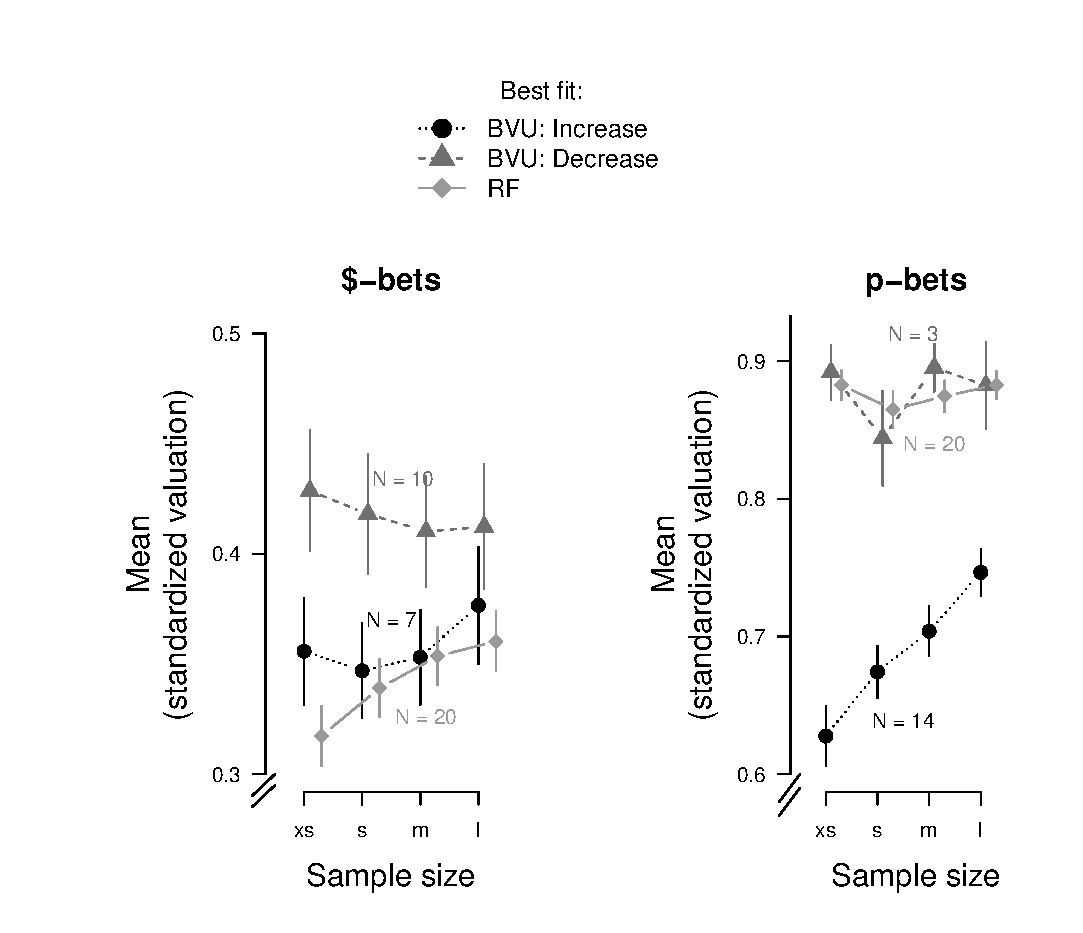
\includegraphics[width=.8\linewidth, keepaspectratio]{groupqual2_stand.eps}
  \caption{\textcolor{blue}{Mean valuations (standardized per gamble between 0 and 1) of people who were best fit by the Bayesian value updating (BVU) model (black and dark gray) and the relative frequency (RF) model (light gray). Depending on whether the BVU model predicted an increase (black) or a decrease (dark gray) in valuations with growing sample size, separately for \$-bets and p-bets we split Bayesian learners into two groups (Increase and Decrease). $N$ describes on how many people's data the means are based. Error bars indicate the standard error of the mean. Sample sizes: xs = extra small; s = small; m = medium; l = large. }}
  \label{fig:qual2}
\end{figure}



\subsubsection{Effect of gamble type and sampling order}
In line with Study 1, the mean and median ratings in Table \ref{table:meansStudy3} show higher valuations for \$-bets (Gambles 1--3) than for p-bets (Gambles 4--6)  even if the gambles had the same expected value (BF\textsubscript{10} \textgreater 1,000). We did not find evidence for any recency or primacy effects. $\mathrm{M}\textsubscript{0}$, which predicts valuations as a function of the factor gamble (1--6), was slightly preferred over models that also include the mean of the first half of the observed samples ($\mathrm{M}\textsubscript{1}$) or the mean of the second half of the observed samples ($\mathrm{M}\textsubscript{2}$) as predictors ($BF\textsubscript{01} = 3.4$, $BF\textsubscript{02} = 1.9$). 

\subsubsection{Confidence ratings}
The mean confidence ratings in the extra small, small, medium, and large sample-size categories were xs = 4.01 ($SD = 1.23$); s = 4.09, ($SD = 1.14$); m = 4.04 ($SD = 1.19)$; and l = 4.16 ($SD = 1.19$). $\mathrm{M}\textsubscript{0}$, which predicts confidence rating as a function of just a random participant effect, was again preferred over a model that also includes sample-size category as predictor ($BF\textsubscript{01} = 11.2$). 

\textcolor{blue}{Considering only those data sets that were best described by the BVU model, mean confidence ratings descriptively increased as a function of  sample size (mean confidence ratings: xs = $3.87$, $SD = 1.27$; s = $3.91$, $SD = 1.15$; m = $3.93$, $SD = 1.13$; l = $4$, $SD = 1.24$). %xs = $3.84$, $SD = 1.31$; s = $3.95$, $SD = 1.16$; m = $4.02$, $SD = 1.13$; l = $4.1$, $SD = 1.28$).
However, this finding was not reliable as the simpler model that predicts no influence of sample size was still preferred over the model that predicts an effect of sample size ($BF\textsubscript{01} = 77$). Similar to in Study 1, the data sets that were quantitatively and qualitatively best described by the RF model did not show an effect of sample size (mean confidence ratings: xs = $4.05$, $SD = 1.19$; s = $4.17$, $SD = 1.1$; m = $4.06$, $SD = 1.22$; l = $4.19$, $SD = 1.14$; $BF\textsubscript{01} = 45$).
}
%xs = $4.04$, $SD = 1.19$; s = $4.14$, $SD = 1.09$; m = $4.02$, $SD = 1.21$; l = $4.13$, $SD = 1.13$; $BF\textsubscript{01} = 72$).
\subsubsection{Description versus experience}

Table \ref{table:meansStudy3} displays the mean and median valuations from experience and from description. It also shows the difference between the mean valuations in the experience and description conditions (column D--E, separately for different sample sizes). 

In line with Study 1, valuations made from experience and description differed. Participants valued experienced \$-bets higher than described \$-bets. In contrast, participants valued described p-bets higher than experienced p-bets. These observations are again in line with the assumption that the probabilities of rare events were overweighted in both conditions, and that this effect was more pronounced for valuations from experience.

Similar to in Study 1, the Bayes factors (rightmost column of Table \ref{table:meansStudy3}) generally suggest a difference between description and experience. However, the finding is, especially for p-bets, less pronounced than in Study 1. Again, the gap is in contrast to the classic D--E gap reported in the decision-making literature.

Participants' mean confidence in valuations from description was 3.99 ($SD = 1.12$). Only for large sample sizes were participants more confident about their valuations from experience than they were about valuations from description ($BF\textsubscript{10} = 53$). There is no evidence for this effect for extra small ($BF\textsubscript{10} = 0.1$), small ($BF\textsubscript{10} = 0.7$), or medium ($BF\textsubscript{10} = 0.1$) sample sizes.
\subsection{Discussion of Study 2}
Study 2 tested whether the results of Study 1 are generalizable to typical sampling paradigms where people have to learn the outcome values from experience. The results of Studies 1 and 2 are remarkably similar: Participants behaved as if they overweighted rare events, when making valuations from both experience and description. In line with Study 1, we found that people could be classified as Bayesian and frequentist learners.

\section{General Discussion}
We studied how sample sizes influence people's valuations of risky gambles in two studies. Whereas in Study 1 the possible gain amount was known before people started sampling, in Study 2 the gain amount had to be learned through sampling. The main goal of these studies was to investigate how people form preferences from experience by comparing gamble valuations after having observed different numbers of outcomes, that is, after encountering different sample sizes. Further, we studied how valuations differ when based on description versus experience. 

%In both Studies, participants behaved as if they overweight rare events from description \textit{and} experience. Behavior in line with overweighting of rare events was even stronger for valuations from experience than for valuations from description: An effect that contrasts with the D--E gap that was described in the choice literature \citep{Hertwig2004}. 

\subsection{Belief in the Law of Small Numbers Versus Bayesian Updating}
Across participants, Studies 1 and 2 showed that the number of samples people drew did not influence their valuations of gambles from experience. People's confidence in valuations was also constant across sample sizes. 

It has been previously shown that people believe in the representativeness of short sequences of outcomes \citep{Griffin1992, Tversky1971}. The RF model that uses relative frequencies of observed outcomes as probability estimates captures this logic. Accordingly, people attend  only to the relative frequency of outcomes when they form gamble valuations and neglect the size of the samples. The model best described the behavior of \textcolor{blue}{30\%} of the participants in Study 1 and \textcolor{blue}{50\%} of the participants in Study 2, which suggests that a substantial proportion of people believe in the law of small numbers. This finding helps explain why people often do not sample much in experience-based tasks: If people believe that a short sequence of outcomes represents a prospect's outcome distribution comprehensively, they do not need to sample much, as they believe that sampling more will not yield new information. 

However, not all participants were best described by the RF model: \textcolor{blue}{65\%}
of the participants in Study 1 and \textcolor{blue}{42.5\%} of the participants in Study 2 were classified as Bayesian learners. Such people treat sample size as information about the uncertainty that the sample sequence entails. As sample size grows, people's prior beliefs about the outcome probabilities have a decreasing impact and valuations of gambles change accordingly. 

Generally, the classification of people into two different subgroups suggests that people use different strategies when they update information from experience. 
%This classification is supported by people's confidence judgments: When we analyzed confidence judgments separately for people who were classified as believers in the law of small numbers and Bayesian learners, we found that only Bayesian learners were more confident about their judgments for larger than for smaller samples. 
% Indeed, when we plotted the mean valuations of participants best described by each model, we see that the data qualitatively differ (compare Figure \ref{fig:qual1} and \ref{fig:qual2}). While valuations of people best fit by the Bayesian model change as a function of sample size, valuations of people best fit by the RF model do not change systematically. 
The question arises of why some people behave according to Bayesian principles and others do not. Future research should focus on examining what factors influence whether people behave according to Bayesian principles. One possible candidate that mediates what strategy people use is numerical literacy. Previous research has, for instance, shown that numerical literacy correlates with performance in Bayesian reasoning tasks \citep{Brase2017}. 

\subsubsection{The role of prior beliefs} 
\textcolor{blue}{The BVU model assumes that people start sampling with a prior belief about how large the gain probability is. Here, we compared four different prior beliefs: first, a uniform prior that described the belief that all possible gain probabilities are equally likely; second, a bimodal prior representing the belief that the gain probabilities are either very low or very high; third, a gain prior representing the belief that gain probabilities are very high, and fourth, a loss prior representing the belief that gain probabilities are very low. Qualitatively, we showed that valuations of Bayesian learners also on the aggregate level either decreased or increased as predicted by the individually best fitting prior. Yet, across both studies, the evidence supporting an influence of sample size on valuations is much stronger for p-bets than for \$-bets. For the latter, across both studies, roughly the same number of people were best fit with a prior belief suggesting that valuations increase with growing sample size and with a prior beliefs suggesting that valuations decrease with growing sample size. Due to this split, the number of participants per group was very low, which further reduced the group sizes. This implies low statistical power.}

\textcolor{blue}{
Many Bayesian learners (8 of 26, 30\% in Study 1 and 7 of 17, 41\% in Study 2) were best described with the loss prior. A loss prior belief predicts that with growing sample sizes, valuations slightly increase for \$-bets and more strongly increase for p-bets (cf. Figure \ref{fig:sensi}). This prediction is in line with our findings that changes in valuations are more pronounced for \$-bets than for p-bets. A slightly different explanation for the behavior of people best fit with the BVU model and a loss prior is that not sample size but the absolute number of observed gains influences valuations. The more gains people observe and the larger the gains are, the more attractive a gamble may be.  Applied most strictly, this hypothesis would suggest larger increases in valuations with growing sample size for \$-bets than for p-bets, as the gain amount in \$-bets is higher. Future research could test this hypothesis, for instance, by investigating valuations for gambles presented with even larger sample sizes. The Bayesian model predicts that with very large sample sizes, selling prices approach people's true selling prices. However, if the absolute number of gains influences selling prices, selling prices should keep increasing as the absolute observed number of gains increases.} %Further, future research should test whether such a hypothesis can explain the valuations of Frequentists learners in Study 2, who --for \$-bets and on the aggregate level-- made higher valuations for larger than smaller sample sizes. 

\textcolor{blue}{
Here, we have assumed that over the course of the experiment and across different gambles, people's prior beliefs do not change. However, recent research suggests that knowing the gain amount elicits a more informed prior belief about the probability. Under uncertainty, people's beliefs about gain probabilities are informed by the gain amount: Large gains are believed to be less likely than small gains when no other information about a gamble than the gain amount is given \citep{Pleskac2014, Hoffart2018}. If in our studies people indeed used gain amounts as predictors of the probability and integrated this information with their samples, this can explain why we see only a small effect of sample size on gamble valuations. This is because in our experimental design large gains were indeed less likely than small gains. Thus, it corresponded to the probability--reward pattern that people might presuppose. If people start sampling with prior probability beliefs that correspond closely to the real outcome probabilities, new incoming information does not shift probability beliefs as dramatically as when the prior beliefs are uninformed (e.g., uniform priors). Future research could investigate this hypothesis, for instance, by investigation how sample size influences valuations in \textit{nonrepresentative} environments, such as environments where the size of a reward/gain is uncorrelated with the probability that it occurs. }

\subsection{Description Versus Experience in Choice and Valuation}
In risky choice tasks, people have been found to behave as if they overweight rare events from description and underweight rare events from experience. In our valuation tasks participants behaved as if they overweighted rare events from both description and experience. Thus, our findings are not in line with the classic D--E gap.

Here, it is noteworthy that in contrast to experience-based choice tasks, in our valuation task, participants only had to focus on one gamble in each trial. This task structure differs from two-gamble choice tasks. This difference in structure might elicit different cognitive processes. Indeed, \cite{Lichtenstein1971} showed that people's preferences based on description can be reversed when elicited by value judgments rather than choices: Someone who chooses Gamble A over Gamble B might still assign a higher value to Gamble B than to Gamble A. One of the first explorations of preference reversals in valuations from experience was done by \cite{Golan2014}. They reported a difference between valuations from description and valuations from experience. Yet, this difference pointed in a direction opposite to our findings: Participants overweighted rare events more strongly when doing so from description than from experience. There is, however, a crucial difference between our experimental design and the experimental design of \cite{Golan2014}. We presented representative sample sequences, whereas they allowed participants to draw as many samples as they wished. As we argued in the Introduction, in free-sampling paradigms, the experienced relative frequencies of outcomes do not necessarily match the underlying probability. Such sampling error might have contributed to the difference in the results. 
Alternatively, the difference could reflect that information is processed differently in free- and forced-sampling paradigms. For instance, people may pay more attention to a sampled outcome that resulted from a voluntary sampling decision than to a sampled outcome that resulted from a forced sampling decision.

\subsubsection{Buying versus selling prices}
In our experiments, we assessed preferences by asking people for selling prices for gambles. 
The endowment effect describes that people attach higher value to goods when they sell them than when they buy them \citep{Thaler1980}. \cite{Pachur2012} demonstrated this endowment effect in an experience-based task. It would be interesting to replicate our experiments with buying instead of selling prices and more rigorously compare the results with buying and selling prices from description. However, this was beyond the scope of the present study. Here, our main focus was to investigate whether preferences are influenced by sample sizes. This question can be answered independently of response format. Irrespective of whether people are asked for selling prices or buying prices or make repeated choices, the Bayesian model predicts an effect of sample size on valuations. 

\subsubsection{Confidence in valuations from description and experience}
People were more confident with their gamble valuations from experience than from description. This finding is remarkable given that from a normative perspective one could argue that people feel more confident when making valuations from description than when making valuations from experience. This is because valuations from description do not entail any uncertainty about the outcome distributions, whereas valuations from experience may entail such uncertainty.

Our findings do support research by \cite{Bradbury2014}. They reported that people who made investment decisions in the laboratory felt better informed and were more confident about their decisions from experience than those from description.
Potentially, people perceive and process experienced information differently from described information \citep{Kahneman2009}: 
While information that is described is more abstract, experienced information has direct salience or impact. When people draw a sample, they not only observe the outcome but also experience emotional reactions resulting from that observation. Thus, people do not only learn plain facts about the outcome distribution; they also gain a more vivid understanding of this distribution. This more concrete understanding of the gamble can help people access their preferences and thus creates higher confidence in valuations.



%\subsection{Conclusion}
%In this study, we investigated how people form  preferences from experience. Our results offer a new perspective on the finding that people sample very little when forming preferences from experience: A substantial proportion of people appear to believe in the law of small numbers; that is, their valuations do not change as a function of sample size. 



\bibliography{refJanine}

%\section{Footnotes}



%Kahnemann (2009): In fact, people are poor forecasters of their future emotions and future tastes—they need help in this task—and I believe that one of the responsibilities offinancial advisors should be to pro-vide that help.

\end{document}


% Please see the package documentation for more information
% on the APA6 document class:
%
% http://www.ctan.org/pkg/apa6
%